% =============================================================================
% 04-registers-instructions-notes.tex — Lecture Notes for Week 4:
% Register & Stack Organization, Instruction Set & Formats,
% Instruction Cycle, Types of Operands
%
% DERIVED ARTIFACT. Source of truth: Slides/CS401/04-registers-instructions.tex.
% Generated by /lecture-notes; do not hand-edit content independently of the
% Beamer source without re-running /qa-notes afterward (single-source-of-truth.md).
% Structured as a textbook chapter (numbered sections/figures/examples,
% topic-organized rather than a frame-by-frame transcript) per the project's
% textbook-chapter convention for Notes.
%
% Anchor reading: Mano, Computer System Architecture, 3rd ed. — Sec. 8-1
%                 (CPU structure, p.241), Sec. 8-2 (general register
%                 organization, p.242), Fig. 5-4 (common bus system, p.129),
%                 Table 8-1 (SELA/SELB/SELD, p.243), Sec. 8-3 (stack
%                 organization, p.247-248), Sec. 8-4 (instruction formats,
%                 p.255) — page-cited from
%                 master_supporting_docs/CS401/supporting_books/Mano1993/index.md,
%                 built and verified 2026-08-06.
%                 Hamacher, Computer Organization, 5th ed., Ch. 7 (instruction
%                 cycle, types of operands) — cited at chapter level only;
%                 this course's Hamacher2002 index does not exist yet.
%                 Patterson & Hennessy, Computer Organization and Design, ARM
%                 Edition (PattersonHennessy2017) — Sec. 2.3 (operands of the
%                 computer hardware, p.67), Sec. 2.5 (representing instructions,
%                 p.82), Sec. 2.7 (instructions for making decisions, p.93) —
%                 page-cited from
%                 master_supporting_docs/CS401/supporting_books/PattersonHennessy2017/index.md,
%                 built 2026-08-07.
%
% Compile with: cd Notes/CS401 &&
%   TEXINPUTS=../../Preambles;$TEXINPUTS xelatex -interaction=nonstopmode 04-registers-instructions-notes.tex
%   BIBINPUTS=../..;$BIBINPUTS bibtex 04-registers-instructions-notes
%   TEXINPUTS=../../Preambles;$TEXINPUTS xelatex -interaction=nonstopmode 04-registers-instructions-notes.tex  (x2)
% =============================================================================

\documentclass[11pt]{article}
\usepackage[margin=1in]{geometry}
% =============================================================================
% Preambles/header.tex — shared LaTeX/Beamer preamble for this project
%
% Use from a Beamer lecture by prepending:
%     % =============================================================================
% Preambles/header.tex — shared LaTeX/Beamer preamble for this project
%
% Use from a Beamer lecture by prepending:
%     % =============================================================================
% Preambles/header.tex — shared LaTeX/Beamer preamble for this project
%
% Use from a Beamer lecture by prepending:
%     \input{header}
% and compiling with TEXINPUTS=../Preambles:$TEXINPUTS (the /compile-latex
% skill does this automatically).
%
% PALETTE CONTRACT. Color names defined here MUST match the names in
% Quarto/theme-template.scss so Beamer and Quarto renderings use the same
% palette. The scripts/check-palette-sync.sh script enforces this.
%
% To customize: edit the HEX values below AND the matching $variable in
% Quarto/theme-template.scss, then run scripts/check-palette-sync.sh.
%
% TITLE PAGE. A formal, serif (Libertine) title-page template is defined in
% the Beamer-only block below (\setbeamertemplate{title page}) -- title,
% subtitle, a thin gold rule, then \author/\institute/\date. Frametitle and
% body text remain on Beamer's sans-serif default. No SCSS counterpart is
% needed for this (font/layout only, no new colors).
% =============================================================================

% -----------------------------------------------------------------------------
% Engine detection + encoding
%
% Our /compile-latex skill uses XeLaTeX, where inputenc is unnecessary and
% can produce encoding warnings. Only load inputenc under pdfTeX.
% -----------------------------------------------------------------------------
\usepackage{iftex}
\ifPDFTeX
  \usepackage[utf8]{inputenc}
\fi

\usepackage{amsmath, amssymb, amsthm}
\usepackage{booktabs}
\usepackage{graphicx}

% -----------------------------------------------------------------------------
% Serif face for the title page (formal/academic look). Linux Libertine is
% XeLaTeX- and pdfTeX-safe and redefines \rmdefault, so \rmfamily picks it up
% everywhere \rmfamily is used explicitly. Body text and frametitles stay on
% Beamer's own sans-serif default (unaffected) -- only the title-page
% \setbeamerfont{...} overrides below opt in to \rmfamily.
% -----------------------------------------------------------------------------
\usepackage{libertine}

% -----------------------------------------------------------------------------
% PALETTE — mirrors Quarto/theme-template.scss variable names.
% Load xcolor and define colors BEFORE anything that references them
% (notably hyperref, hypersetup, and the Beamer color assignments).
% -----------------------------------------------------------------------------
\usepackage{xcolor}

\definecolor{primary-blue}{HTML}{012169}      % headings, accents
\definecolor{primary-gold}{HTML}{B9975B}      % emphasis, borders
\definecolor{highlight-yellow}{HTML}{F2A900}  % markers, alerts
\definecolor{light-bg}{HTML}{E8EDF5}          % title / section backgrounds
\definecolor{jet}{HTML}{1A1A1A}               % body text

% Semantic colors (used in diagrams and annotations)
\definecolor{positive}{HTML}{15803D}          % good / observed / identified
\definecolor{negative}{HTML}{B91C1C}          % bad / problematic / bias
\definecolor{neutral}{HTML}{525252}           % reference / context

% Highlight accents (match .hi-* classes in the SCSS)
\definecolor{hi-slate}{HTML}{314F4F}
\definecolor{hi-green}{HTML}{2E8B57}
\definecolor{hi-red}{HTML}{C41E3A}

% Semantic aliases so skill templates and snippets can write
% \textcolor{accent}{...} without hard-coding "primary-blue".
\colorlet{accent}{primary-blue}
\colorlet{accent2}{primary-gold}

% -----------------------------------------------------------------------------
% Hyperref — loaded AFTER xcolor + palette so link colors resolve.
% -----------------------------------------------------------------------------
\usepackage{hyperref}
\hypersetup{colorlinks=true, linkcolor=primary-blue, urlcolor=primary-blue,
            citecolor=primary-blue, pdfborder={0 0 0}}

% -----------------------------------------------------------------------------
% Course code — set once per deck (after \input{header}, before \begin{document})
% via \coursecode{CS401}. Shown in the footer on every slide so a deck's course
% is identifiable without opening the title page. Empty by default.
% -----------------------------------------------------------------------------
\makeatletter
\newcommand{\coursecode}[1]{\gdef\@coursecodetext{#1}}
\gdef\@coursecodetext{}
\makeatother

% -----------------------------------------------------------------------------
% Beamer theme assignments (only apply under Beamer).
%
% We detect Beamer via \@ifclassloaded{beamer}, which is the documented,
% non-internal way. This must be wrapped in \makeatletter/\makeatother
% because \@ifclassloaded contains an @-catcode character.
% -----------------------------------------------------------------------------
\makeatletter
\@ifclassloaded{beamer}{%
  \usefonttheme{professionalfonts}
  \setbeamercolor{structure}{fg=primary-blue}
  \setbeamercolor{frametitle}{fg=primary-blue}
  \setbeamercolor{title}{fg=primary-blue}
  \setbeamercolor{subtitle}{fg=primary-gold}
  \setbeamercolor{author}{fg=primary-blue}
  \setbeamercolor{institute}{fg=neutral}
  \setbeamercolor{date}{fg=primary-gold}
  \setbeamercolor{itemize item}{fg=primary-blue}
  \setbeamercolor{itemize subitem}{fg=primary-gold}
  \setbeamercolor{alerted text}{fg=primary-gold}
  \setbeamercolor{block title}{fg=white, bg=primary-blue}
  \setbeamercolor{block body}{bg=light-bg}
  % Semantic block variants: block=definition/concept (blue), exampleblock=
  % worked example (green/positive), alertblock=key takeaway or caution (gold).
  % Keep to <=2 colored boxes per slide across ALL three variants (INV-7).
  \setbeamercolor{block title example}{fg=white, bg=positive}
  \setbeamercolor{block body example}{bg=light-bg}
  \setbeamercolor{block title alerted}{fg=white, bg=primary-gold}
  \setbeamercolor{block body alerted}{bg=light-bg}

  % ---------------------------------------------------------------------------
  % Formal title page: serif (Libertine, via \rmfamily) for title-page
  % elements only. Body text, itemize, and frametitle are intentionally left
  % on Beamer's sans-serif default -- \usebeamerfont{title} is also what
  % \transitionslide (below) uses for its big centered text, so section
  % transitions pick up the same serif treatment for free.
  % ---------------------------------------------------------------------------
  \setbeamerfont{title}{family=\rmfamily, series=\bfseries, size=\Large}
  \setbeamerfont{subtitle}{family=\rmfamily, shape=\itshape, size=\normalsize}
  \setbeamerfont{author}{family=\rmfamily, size=\normalsize}
  \setbeamerfont{institute}{family=\rmfamily, size=\scriptsize}
  \setbeamerfont{date}{family=\rmfamily, size=\scriptsize}

  \setbeamertemplate{title page}{
    \vfill
    \begin{center}
      {\usebeamerfont{title}\usebeamercolor[fg]{title}\inserttitle\par}
      \vspace{0.15cm}
      {\usebeamerfont{subtitle}\usebeamercolor[fg]{subtitle}\insertsubtitle\par}
      \vspace{0.45cm}
      {\color{primary-gold}\rule{0.42\textwidth}{0.6pt}\par}
      \vspace{0.45cm}
      {\usebeamerfont{author}\usebeamercolor[fg]{author}\insertauthor\par}
      \vspace{0.35cm}
      {\usebeamerfont{institute}\usebeamercolor[fg]{institute}\insertinstitute\par}
      \vspace{0.35cm}
      {\usebeamerfont{date}\usebeamercolor[fg]{date}\insertdate\par}
    \end{center}
    \vfill
  }

  % Minimal footer: course code (left) + page X / N (right), no navigation clutter
  \setbeamertemplate{navigation symbols}{}
  \setbeamertemplate{footline}{%
    \color{neutral}\footnotesize\hspace{0.7em}\@coursecodetext\hfill
    \insertframenumber/\inserttotalframenumber\hspace{0.7em}\vspace{0.3em}}
}{}
\makeatother

% -----------------------------------------------------------------------------
% TikZ setup — libraries the snippet gallery uses
% -----------------------------------------------------------------------------
\usepackage{tikz}
\usetikzlibrary{arrows.meta, positioning, calc, decorations.pathreplacing,
                fit, shapes.geometric, backgrounds}

% Shared TikZ styles — snippets and hand-written diagrams can pick these up
% via `\begin{tikzpicture}[every node/.style={...}]` or by naming specific
% styles (e.g., `\node[dag-node] (X) at (0,0) {X};`).
\tikzset{
  % Node styles for causal DAGs and similar
  dag-node/.style = {
    draw=primary-blue, fill=light-bg, rounded corners=2pt,
    minimum width=1.2cm, minimum height=0.9cm, align=center, font=\small
  },
  decision-node/.style = {
    draw=primary-gold, fill=white, diamond, aspect=1.8,
    minimum width=1.8cm, minimum height=1.2cm, align=center, font=\small,
    inner sep=1pt
  },
  % Edge styles — observed vs counterfactual
  observed-edge/.style = {-{Latex[length=2.5mm]}, thick, draw=jet},
  counterfactual-edge/.style = {-{Latex[length=2.5mm]}, thick, draw=neutral, dashed},
  confound-edge/.style = {-{Latex[length=2.5mm]}, thick, draw=negative, dashed},
  % Data-point styles for plots
  observed-dot/.style = {fill=primary-blue, draw=primary-blue, circle, inner sep=1.2pt},
  counterfactual-dot/.style = {fill=white, draw=neutral, circle, inner sep=1.2pt}
}

% -----------------------------------------------------------------------------
% Convenience macros
% -----------------------------------------------------------------------------
\newcommand{\muted}[1]{\textcolor{neutral}{#1}}
\newcommand{\key}[1]{\textcolor{primary-gold}{\textbf{#1}}}
\newcommand{\good}[1]{\textcolor{positive}{#1}}
\newcommand{\bad}[1]{\textcolor{negative}{#1}}

% Standout frame macro: full-bleed dark background for section transitions.
% Beamer-only (uses \begin{frame}/\setbeamercolor/\usebeamerfont) -- do not
% call from an article-class file (e.g. Notes/<CODE>/*-notes.tex). \muted,
% \key, \good, \bad, and \coursecode above are plain xcolor/gdef and are
% safe to use from either class; verified when Notes/article-class support
% was added.
% Expand: \transitionslide{Your transition title}
\newcommand{\transitionslide}[1]{%
  \begingroup
  \setbeamercolor{background canvas}{bg=primary-blue}
  \begin{frame}[plain]
    \centering
    \vfill
    {\usebeamerfont{title}\color{white}\Large #1\par}
    \vfill
  \end{frame}
  \endgroup
}

% and compiling with TEXINPUTS=../Preambles:$TEXINPUTS (the /compile-latex
% skill does this automatically).
%
% PALETTE CONTRACT. Color names defined here MUST match the names in
% Quarto/theme-template.scss so Beamer and Quarto renderings use the same
% palette. The scripts/check-palette-sync.sh script enforces this.
%
% To customize: edit the HEX values below AND the matching $variable in
% Quarto/theme-template.scss, then run scripts/check-palette-sync.sh.
%
% TITLE PAGE. A formal, serif (Libertine) title-page template is defined in
% the Beamer-only block below (\setbeamertemplate{title page}) -- title,
% subtitle, a thin gold rule, then \author/\institute/\date. Frametitle and
% body text remain on Beamer's sans-serif default. No SCSS counterpart is
% needed for this (font/layout only, no new colors).
% =============================================================================

% -----------------------------------------------------------------------------
% Engine detection + encoding
%
% Our /compile-latex skill uses XeLaTeX, where inputenc is unnecessary and
% can produce encoding warnings. Only load inputenc under pdfTeX.
% -----------------------------------------------------------------------------
\usepackage{iftex}
\ifPDFTeX
  \usepackage[utf8]{inputenc}
\fi

\usepackage{amsmath, amssymb, amsthm}
\usepackage{booktabs}
\usepackage{graphicx}

% -----------------------------------------------------------------------------
% Serif face for the title page (formal/academic look). Linux Libertine is
% XeLaTeX- and pdfTeX-safe and redefines \rmdefault, so \rmfamily picks it up
% everywhere \rmfamily is used explicitly. Body text and frametitles stay on
% Beamer's own sans-serif default (unaffected) -- only the title-page
% \setbeamerfont{...} overrides below opt in to \rmfamily.
% -----------------------------------------------------------------------------
\usepackage{libertine}

% -----------------------------------------------------------------------------
% PALETTE — mirrors Quarto/theme-template.scss variable names.
% Load xcolor and define colors BEFORE anything that references them
% (notably hyperref, hypersetup, and the Beamer color assignments).
% -----------------------------------------------------------------------------
\usepackage{xcolor}

\definecolor{primary-blue}{HTML}{012169}      % headings, accents
\definecolor{primary-gold}{HTML}{B9975B}      % emphasis, borders
\definecolor{highlight-yellow}{HTML}{F2A900}  % markers, alerts
\definecolor{light-bg}{HTML}{E8EDF5}          % title / section backgrounds
\definecolor{jet}{HTML}{1A1A1A}               % body text

% Semantic colors (used in diagrams and annotations)
\definecolor{positive}{HTML}{15803D}          % good / observed / identified
\definecolor{negative}{HTML}{B91C1C}          % bad / problematic / bias
\definecolor{neutral}{HTML}{525252}           % reference / context

% Highlight accents (match .hi-* classes in the SCSS)
\definecolor{hi-slate}{HTML}{314F4F}
\definecolor{hi-green}{HTML}{2E8B57}
\definecolor{hi-red}{HTML}{C41E3A}

% Semantic aliases so skill templates and snippets can write
% \textcolor{accent}{...} without hard-coding "primary-blue".
\colorlet{accent}{primary-blue}
\colorlet{accent2}{primary-gold}

% -----------------------------------------------------------------------------
% Hyperref — loaded AFTER xcolor + palette so link colors resolve.
% -----------------------------------------------------------------------------
\usepackage{hyperref}
\hypersetup{colorlinks=true, linkcolor=primary-blue, urlcolor=primary-blue,
            citecolor=primary-blue, pdfborder={0 0 0}}

% -----------------------------------------------------------------------------
% Course code — set once per deck (after % =============================================================================
% Preambles/header.tex — shared LaTeX/Beamer preamble for this project
%
% Use from a Beamer lecture by prepending:
%     \input{header}
% and compiling with TEXINPUTS=../Preambles:$TEXINPUTS (the /compile-latex
% skill does this automatically).
%
% PALETTE CONTRACT. Color names defined here MUST match the names in
% Quarto/theme-template.scss so Beamer and Quarto renderings use the same
% palette. The scripts/check-palette-sync.sh script enforces this.
%
% To customize: edit the HEX values below AND the matching $variable in
% Quarto/theme-template.scss, then run scripts/check-palette-sync.sh.
%
% TITLE PAGE. A formal, serif (Libertine) title-page template is defined in
% the Beamer-only block below (\setbeamertemplate{title page}) -- title,
% subtitle, a thin gold rule, then \author/\institute/\date. Frametitle and
% body text remain on Beamer's sans-serif default. No SCSS counterpart is
% needed for this (font/layout only, no new colors).
% =============================================================================

% -----------------------------------------------------------------------------
% Engine detection + encoding
%
% Our /compile-latex skill uses XeLaTeX, where inputenc is unnecessary and
% can produce encoding warnings. Only load inputenc under pdfTeX.
% -----------------------------------------------------------------------------
\usepackage{iftex}
\ifPDFTeX
  \usepackage[utf8]{inputenc}
\fi

\usepackage{amsmath, amssymb, amsthm}
\usepackage{booktabs}
\usepackage{graphicx}

% -----------------------------------------------------------------------------
% Serif face for the title page (formal/academic look). Linux Libertine is
% XeLaTeX- and pdfTeX-safe and redefines \rmdefault, so \rmfamily picks it up
% everywhere \rmfamily is used explicitly. Body text and frametitles stay on
% Beamer's own sans-serif default (unaffected) -- only the title-page
% \setbeamerfont{...} overrides below opt in to \rmfamily.
% -----------------------------------------------------------------------------
\usepackage{libertine}

% -----------------------------------------------------------------------------
% PALETTE — mirrors Quarto/theme-template.scss variable names.
% Load xcolor and define colors BEFORE anything that references them
% (notably hyperref, hypersetup, and the Beamer color assignments).
% -----------------------------------------------------------------------------
\usepackage{xcolor}

\definecolor{primary-blue}{HTML}{012169}      % headings, accents
\definecolor{primary-gold}{HTML}{B9975B}      % emphasis, borders
\definecolor{highlight-yellow}{HTML}{F2A900}  % markers, alerts
\definecolor{light-bg}{HTML}{E8EDF5}          % title / section backgrounds
\definecolor{jet}{HTML}{1A1A1A}               % body text

% Semantic colors (used in diagrams and annotations)
\definecolor{positive}{HTML}{15803D}          % good / observed / identified
\definecolor{negative}{HTML}{B91C1C}          % bad / problematic / bias
\definecolor{neutral}{HTML}{525252}           % reference / context

% Highlight accents (match .hi-* classes in the SCSS)
\definecolor{hi-slate}{HTML}{314F4F}
\definecolor{hi-green}{HTML}{2E8B57}
\definecolor{hi-red}{HTML}{C41E3A}

% Semantic aliases so skill templates and snippets can write
% \textcolor{accent}{...} without hard-coding "primary-blue".
\colorlet{accent}{primary-blue}
\colorlet{accent2}{primary-gold}

% -----------------------------------------------------------------------------
% Hyperref — loaded AFTER xcolor + palette so link colors resolve.
% -----------------------------------------------------------------------------
\usepackage{hyperref}
\hypersetup{colorlinks=true, linkcolor=primary-blue, urlcolor=primary-blue,
            citecolor=primary-blue, pdfborder={0 0 0}}

% -----------------------------------------------------------------------------
% Course code — set once per deck (after \input{header}, before \begin{document})
% via \coursecode{CS401}. Shown in the footer on every slide so a deck's course
% is identifiable without opening the title page. Empty by default.
% -----------------------------------------------------------------------------
\makeatletter
\newcommand{\coursecode}[1]{\gdef\@coursecodetext{#1}}
\gdef\@coursecodetext{}
\makeatother

% -----------------------------------------------------------------------------
% Beamer theme assignments (only apply under Beamer).
%
% We detect Beamer via \@ifclassloaded{beamer}, which is the documented,
% non-internal way. This must be wrapped in \makeatletter/\makeatother
% because \@ifclassloaded contains an @-catcode character.
% -----------------------------------------------------------------------------
\makeatletter
\@ifclassloaded{beamer}{%
  \usefonttheme{professionalfonts}
  \setbeamercolor{structure}{fg=primary-blue}
  \setbeamercolor{frametitle}{fg=primary-blue}
  \setbeamercolor{title}{fg=primary-blue}
  \setbeamercolor{subtitle}{fg=primary-gold}
  \setbeamercolor{author}{fg=primary-blue}
  \setbeamercolor{institute}{fg=neutral}
  \setbeamercolor{date}{fg=primary-gold}
  \setbeamercolor{itemize item}{fg=primary-blue}
  \setbeamercolor{itemize subitem}{fg=primary-gold}
  \setbeamercolor{alerted text}{fg=primary-gold}
  \setbeamercolor{block title}{fg=white, bg=primary-blue}
  \setbeamercolor{block body}{bg=light-bg}
  % Semantic block variants: block=definition/concept (blue), exampleblock=
  % worked example (green/positive), alertblock=key takeaway or caution (gold).
  % Keep to <=2 colored boxes per slide across ALL three variants (INV-7).
  \setbeamercolor{block title example}{fg=white, bg=positive}
  \setbeamercolor{block body example}{bg=light-bg}
  \setbeamercolor{block title alerted}{fg=white, bg=primary-gold}
  \setbeamercolor{block body alerted}{bg=light-bg}

  % ---------------------------------------------------------------------------
  % Formal title page: serif (Libertine, via \rmfamily) for title-page
  % elements only. Body text, itemize, and frametitle are intentionally left
  % on Beamer's sans-serif default -- \usebeamerfont{title} is also what
  % \transitionslide (below) uses for its big centered text, so section
  % transitions pick up the same serif treatment for free.
  % ---------------------------------------------------------------------------
  \setbeamerfont{title}{family=\rmfamily, series=\bfseries, size=\Large}
  \setbeamerfont{subtitle}{family=\rmfamily, shape=\itshape, size=\normalsize}
  \setbeamerfont{author}{family=\rmfamily, size=\normalsize}
  \setbeamerfont{institute}{family=\rmfamily, size=\scriptsize}
  \setbeamerfont{date}{family=\rmfamily, size=\scriptsize}

  \setbeamertemplate{title page}{
    \vfill
    \begin{center}
      {\usebeamerfont{title}\usebeamercolor[fg]{title}\inserttitle\par}
      \vspace{0.15cm}
      {\usebeamerfont{subtitle}\usebeamercolor[fg]{subtitle}\insertsubtitle\par}
      \vspace{0.45cm}
      {\color{primary-gold}\rule{0.42\textwidth}{0.6pt}\par}
      \vspace{0.45cm}
      {\usebeamerfont{author}\usebeamercolor[fg]{author}\insertauthor\par}
      \vspace{0.35cm}
      {\usebeamerfont{institute}\usebeamercolor[fg]{institute}\insertinstitute\par}
      \vspace{0.35cm}
      {\usebeamerfont{date}\usebeamercolor[fg]{date}\insertdate\par}
    \end{center}
    \vfill
  }

  % Minimal footer: course code (left) + page X / N (right), no navigation clutter
  \setbeamertemplate{navigation symbols}{}
  \setbeamertemplate{footline}{%
    \color{neutral}\footnotesize\hspace{0.7em}\@coursecodetext\hfill
    \insertframenumber/\inserttotalframenumber\hspace{0.7em}\vspace{0.3em}}
}{}
\makeatother

% -----------------------------------------------------------------------------
% TikZ setup — libraries the snippet gallery uses
% -----------------------------------------------------------------------------
\usepackage{tikz}
\usetikzlibrary{arrows.meta, positioning, calc, decorations.pathreplacing,
                fit, shapes.geometric, backgrounds}

% Shared TikZ styles — snippets and hand-written diagrams can pick these up
% via `\begin{tikzpicture}[every node/.style={...}]` or by naming specific
% styles (e.g., `\node[dag-node] (X) at (0,0) {X};`).
\tikzset{
  % Node styles for causal DAGs and similar
  dag-node/.style = {
    draw=primary-blue, fill=light-bg, rounded corners=2pt,
    minimum width=1.2cm, minimum height=0.9cm, align=center, font=\small
  },
  decision-node/.style = {
    draw=primary-gold, fill=white, diamond, aspect=1.8,
    minimum width=1.8cm, minimum height=1.2cm, align=center, font=\small,
    inner sep=1pt
  },
  % Edge styles — observed vs counterfactual
  observed-edge/.style = {-{Latex[length=2.5mm]}, thick, draw=jet},
  counterfactual-edge/.style = {-{Latex[length=2.5mm]}, thick, draw=neutral, dashed},
  confound-edge/.style = {-{Latex[length=2.5mm]}, thick, draw=negative, dashed},
  % Data-point styles for plots
  observed-dot/.style = {fill=primary-blue, draw=primary-blue, circle, inner sep=1.2pt},
  counterfactual-dot/.style = {fill=white, draw=neutral, circle, inner sep=1.2pt}
}

% -----------------------------------------------------------------------------
% Convenience macros
% -----------------------------------------------------------------------------
\newcommand{\muted}[1]{\textcolor{neutral}{#1}}
\newcommand{\key}[1]{\textcolor{primary-gold}{\textbf{#1}}}
\newcommand{\good}[1]{\textcolor{positive}{#1}}
\newcommand{\bad}[1]{\textcolor{negative}{#1}}

% Standout frame macro: full-bleed dark background for section transitions.
% Beamer-only (uses \begin{frame}/\setbeamercolor/\usebeamerfont) -- do not
% call from an article-class file (e.g. Notes/<CODE>/*-notes.tex). \muted,
% \key, \good, \bad, and \coursecode above are plain xcolor/gdef and are
% safe to use from either class; verified when Notes/article-class support
% was added.
% Expand: \transitionslide{Your transition title}
\newcommand{\transitionslide}[1]{%
  \begingroup
  \setbeamercolor{background canvas}{bg=primary-blue}
  \begin{frame}[plain]
    \centering
    \vfill
    {\usebeamerfont{title}\color{white}\Large #1\par}
    \vfill
  \end{frame}
  \endgroup
}
, before \begin{document})
% via \coursecode{CS401}. Shown in the footer on every slide so a deck's course
% is identifiable without opening the title page. Empty by default.
% -----------------------------------------------------------------------------
\makeatletter
\newcommand{\coursecode}[1]{\gdef\@coursecodetext{#1}}
\gdef\@coursecodetext{}
\makeatother

% -----------------------------------------------------------------------------
% Beamer theme assignments (only apply under Beamer).
%
% We detect Beamer via \@ifclassloaded{beamer}, which is the documented,
% non-internal way. This must be wrapped in \makeatletter/\makeatother
% because \@ifclassloaded contains an @-catcode character.
% -----------------------------------------------------------------------------
\makeatletter
\@ifclassloaded{beamer}{%
  \usefonttheme{professionalfonts}
  \setbeamercolor{structure}{fg=primary-blue}
  \setbeamercolor{frametitle}{fg=primary-blue}
  \setbeamercolor{title}{fg=primary-blue}
  \setbeamercolor{subtitle}{fg=primary-gold}
  \setbeamercolor{author}{fg=primary-blue}
  \setbeamercolor{institute}{fg=neutral}
  \setbeamercolor{date}{fg=primary-gold}
  \setbeamercolor{itemize item}{fg=primary-blue}
  \setbeamercolor{itemize subitem}{fg=primary-gold}
  \setbeamercolor{alerted text}{fg=primary-gold}
  \setbeamercolor{block title}{fg=white, bg=primary-blue}
  \setbeamercolor{block body}{bg=light-bg}
  % Semantic block variants: block=definition/concept (blue), exampleblock=
  % worked example (green/positive), alertblock=key takeaway or caution (gold).
  % Keep to <=2 colored boxes per slide across ALL three variants (INV-7).
  \setbeamercolor{block title example}{fg=white, bg=positive}
  \setbeamercolor{block body example}{bg=light-bg}
  \setbeamercolor{block title alerted}{fg=white, bg=primary-gold}
  \setbeamercolor{block body alerted}{bg=light-bg}

  % ---------------------------------------------------------------------------
  % Formal title page: serif (Libertine, via \rmfamily) for title-page
  % elements only. Body text, itemize, and frametitle are intentionally left
  % on Beamer's sans-serif default -- \usebeamerfont{title} is also what
  % \transitionslide (below) uses for its big centered text, so section
  % transitions pick up the same serif treatment for free.
  % ---------------------------------------------------------------------------
  \setbeamerfont{title}{family=\rmfamily, series=\bfseries, size=\Large}
  \setbeamerfont{subtitle}{family=\rmfamily, shape=\itshape, size=\normalsize}
  \setbeamerfont{author}{family=\rmfamily, size=\normalsize}
  \setbeamerfont{institute}{family=\rmfamily, size=\scriptsize}
  \setbeamerfont{date}{family=\rmfamily, size=\scriptsize}

  \setbeamertemplate{title page}{
    \vfill
    \begin{center}
      {\usebeamerfont{title}\usebeamercolor[fg]{title}\inserttitle\par}
      \vspace{0.15cm}
      {\usebeamerfont{subtitle}\usebeamercolor[fg]{subtitle}\insertsubtitle\par}
      \vspace{0.45cm}
      {\color{primary-gold}\rule{0.42\textwidth}{0.6pt}\par}
      \vspace{0.45cm}
      {\usebeamerfont{author}\usebeamercolor[fg]{author}\insertauthor\par}
      \vspace{0.35cm}
      {\usebeamerfont{institute}\usebeamercolor[fg]{institute}\insertinstitute\par}
      \vspace{0.35cm}
      {\usebeamerfont{date}\usebeamercolor[fg]{date}\insertdate\par}
    \end{center}
    \vfill
  }

  % Minimal footer: course code (left) + page X / N (right), no navigation clutter
  \setbeamertemplate{navigation symbols}{}
  \setbeamertemplate{footline}{%
    \color{neutral}\footnotesize\hspace{0.7em}\@coursecodetext\hfill
    \insertframenumber/\inserttotalframenumber\hspace{0.7em}\vspace{0.3em}}
}{}
\makeatother

% -----------------------------------------------------------------------------
% TikZ setup — libraries the snippet gallery uses
% -----------------------------------------------------------------------------
\usepackage{tikz}
\usetikzlibrary{arrows.meta, positioning, calc, decorations.pathreplacing,
                fit, shapes.geometric, backgrounds}

% Shared TikZ styles — snippets and hand-written diagrams can pick these up
% via `\begin{tikzpicture}[every node/.style={...}]` or by naming specific
% styles (e.g., `\node[dag-node] (X) at (0,0) {X};`).
\tikzset{
  % Node styles for causal DAGs and similar
  dag-node/.style = {
    draw=primary-blue, fill=light-bg, rounded corners=2pt,
    minimum width=1.2cm, minimum height=0.9cm, align=center, font=\small
  },
  decision-node/.style = {
    draw=primary-gold, fill=white, diamond, aspect=1.8,
    minimum width=1.8cm, minimum height=1.2cm, align=center, font=\small,
    inner sep=1pt
  },
  % Edge styles — observed vs counterfactual
  observed-edge/.style = {-{Latex[length=2.5mm]}, thick, draw=jet},
  counterfactual-edge/.style = {-{Latex[length=2.5mm]}, thick, draw=neutral, dashed},
  confound-edge/.style = {-{Latex[length=2.5mm]}, thick, draw=negative, dashed},
  % Data-point styles for plots
  observed-dot/.style = {fill=primary-blue, draw=primary-blue, circle, inner sep=1.2pt},
  counterfactual-dot/.style = {fill=white, draw=neutral, circle, inner sep=1.2pt}
}

% -----------------------------------------------------------------------------
% Convenience macros
% -----------------------------------------------------------------------------
\newcommand{\muted}[1]{\textcolor{neutral}{#1}}
\newcommand{\key}[1]{\textcolor{primary-gold}{\textbf{#1}}}
\newcommand{\good}[1]{\textcolor{positive}{#1}}
\newcommand{\bad}[1]{\textcolor{negative}{#1}}

% Standout frame macro: full-bleed dark background for section transitions.
% Beamer-only (uses \begin{frame}/\setbeamercolor/\usebeamerfont) -- do not
% call from an article-class file (e.g. Notes/<CODE>/*-notes.tex). \muted,
% \key, \good, \bad, and \coursecode above are plain xcolor/gdef and are
% safe to use from either class; verified when Notes/article-class support
% was added.
% Expand: \transitionslide{Your transition title}
\newcommand{\transitionslide}[1]{%
  \begingroup
  \setbeamercolor{background canvas}{bg=primary-blue}
  \begin{frame}[plain]
    \centering
    \vfill
    {\usebeamerfont{title}\color{white}\Large #1\par}
    \vfill
  \end{frame}
  \endgroup
}

% and compiling with TEXINPUTS=../Preambles:$TEXINPUTS (the /compile-latex
% skill does this automatically).
%
% PALETTE CONTRACT. Color names defined here MUST match the names in
% Quarto/theme-template.scss so Beamer and Quarto renderings use the same
% palette. The scripts/check-palette-sync.sh script enforces this.
%
% To customize: edit the HEX values below AND the matching $variable in
% Quarto/theme-template.scss, then run scripts/check-palette-sync.sh.
%
% TITLE PAGE. A formal, serif (Libertine) title-page template is defined in
% the Beamer-only block below (\setbeamertemplate{title page}) -- title,
% subtitle, a thin gold rule, then \author/\institute/\date. Frametitle and
% body text remain on Beamer's sans-serif default. No SCSS counterpart is
% needed for this (font/layout only, no new colors).
% =============================================================================

% -----------------------------------------------------------------------------
% Engine detection + encoding
%
% Our /compile-latex skill uses XeLaTeX, where inputenc is unnecessary and
% can produce encoding warnings. Only load inputenc under pdfTeX.
% -----------------------------------------------------------------------------
\usepackage{iftex}
\ifPDFTeX
  \usepackage[utf8]{inputenc}
\fi

\usepackage{amsmath, amssymb, amsthm}
\usepackage{booktabs}
\usepackage{graphicx}

% -----------------------------------------------------------------------------
% Serif face for the title page (formal/academic look). Linux Libertine is
% XeLaTeX- and pdfTeX-safe and redefines \rmdefault, so \rmfamily picks it up
% everywhere \rmfamily is used explicitly. Body text and frametitles stay on
% Beamer's own sans-serif default (unaffected) -- only the title-page
% \setbeamerfont{...} overrides below opt in to \rmfamily.
% -----------------------------------------------------------------------------
\usepackage{libertine}

% -----------------------------------------------------------------------------
% PALETTE — mirrors Quarto/theme-template.scss variable names.
% Load xcolor and define colors BEFORE anything that references them
% (notably hyperref, hypersetup, and the Beamer color assignments).
% -----------------------------------------------------------------------------
\usepackage{xcolor}

\definecolor{primary-blue}{HTML}{012169}      % headings, accents
\definecolor{primary-gold}{HTML}{B9975B}      % emphasis, borders
\definecolor{highlight-yellow}{HTML}{F2A900}  % markers, alerts
\definecolor{light-bg}{HTML}{E8EDF5}          % title / section backgrounds
\definecolor{jet}{HTML}{1A1A1A}               % body text

% Semantic colors (used in diagrams and annotations)
\definecolor{positive}{HTML}{15803D}          % good / observed / identified
\definecolor{negative}{HTML}{B91C1C}          % bad / problematic / bias
\definecolor{neutral}{HTML}{525252}           % reference / context

% Highlight accents (match .hi-* classes in the SCSS)
\definecolor{hi-slate}{HTML}{314F4F}
\definecolor{hi-green}{HTML}{2E8B57}
\definecolor{hi-red}{HTML}{C41E3A}

% Semantic aliases so skill templates and snippets can write
% \textcolor{accent}{...} without hard-coding "primary-blue".
\colorlet{accent}{primary-blue}
\colorlet{accent2}{primary-gold}

% -----------------------------------------------------------------------------
% Hyperref — loaded AFTER xcolor + palette so link colors resolve.
% -----------------------------------------------------------------------------
\usepackage{hyperref}
\hypersetup{colorlinks=true, linkcolor=primary-blue, urlcolor=primary-blue,
            citecolor=primary-blue, pdfborder={0 0 0}}

% -----------------------------------------------------------------------------
% Course code — set once per deck (after % =============================================================================
% Preambles/header.tex — shared LaTeX/Beamer preamble for this project
%
% Use from a Beamer lecture by prepending:
%     % =============================================================================
% Preambles/header.tex — shared LaTeX/Beamer preamble for this project
%
% Use from a Beamer lecture by prepending:
%     \input{header}
% and compiling with TEXINPUTS=../Preambles:$TEXINPUTS (the /compile-latex
% skill does this automatically).
%
% PALETTE CONTRACT. Color names defined here MUST match the names in
% Quarto/theme-template.scss so Beamer and Quarto renderings use the same
% palette. The scripts/check-palette-sync.sh script enforces this.
%
% To customize: edit the HEX values below AND the matching $variable in
% Quarto/theme-template.scss, then run scripts/check-palette-sync.sh.
%
% TITLE PAGE. A formal, serif (Libertine) title-page template is defined in
% the Beamer-only block below (\setbeamertemplate{title page}) -- title,
% subtitle, a thin gold rule, then \author/\institute/\date. Frametitle and
% body text remain on Beamer's sans-serif default. No SCSS counterpart is
% needed for this (font/layout only, no new colors).
% =============================================================================

% -----------------------------------------------------------------------------
% Engine detection + encoding
%
% Our /compile-latex skill uses XeLaTeX, where inputenc is unnecessary and
% can produce encoding warnings. Only load inputenc under pdfTeX.
% -----------------------------------------------------------------------------
\usepackage{iftex}
\ifPDFTeX
  \usepackage[utf8]{inputenc}
\fi

\usepackage{amsmath, amssymb, amsthm}
\usepackage{booktabs}
\usepackage{graphicx}

% -----------------------------------------------------------------------------
% Serif face for the title page (formal/academic look). Linux Libertine is
% XeLaTeX- and pdfTeX-safe and redefines \rmdefault, so \rmfamily picks it up
% everywhere \rmfamily is used explicitly. Body text and frametitles stay on
% Beamer's own sans-serif default (unaffected) -- only the title-page
% \setbeamerfont{...} overrides below opt in to \rmfamily.
% -----------------------------------------------------------------------------
\usepackage{libertine}

% -----------------------------------------------------------------------------
% PALETTE — mirrors Quarto/theme-template.scss variable names.
% Load xcolor and define colors BEFORE anything that references them
% (notably hyperref, hypersetup, and the Beamer color assignments).
% -----------------------------------------------------------------------------
\usepackage{xcolor}

\definecolor{primary-blue}{HTML}{012169}      % headings, accents
\definecolor{primary-gold}{HTML}{B9975B}      % emphasis, borders
\definecolor{highlight-yellow}{HTML}{F2A900}  % markers, alerts
\definecolor{light-bg}{HTML}{E8EDF5}          % title / section backgrounds
\definecolor{jet}{HTML}{1A1A1A}               % body text

% Semantic colors (used in diagrams and annotations)
\definecolor{positive}{HTML}{15803D}          % good / observed / identified
\definecolor{negative}{HTML}{B91C1C}          % bad / problematic / bias
\definecolor{neutral}{HTML}{525252}           % reference / context

% Highlight accents (match .hi-* classes in the SCSS)
\definecolor{hi-slate}{HTML}{314F4F}
\definecolor{hi-green}{HTML}{2E8B57}
\definecolor{hi-red}{HTML}{C41E3A}

% Semantic aliases so skill templates and snippets can write
% \textcolor{accent}{...} without hard-coding "primary-blue".
\colorlet{accent}{primary-blue}
\colorlet{accent2}{primary-gold}

% -----------------------------------------------------------------------------
% Hyperref — loaded AFTER xcolor + palette so link colors resolve.
% -----------------------------------------------------------------------------
\usepackage{hyperref}
\hypersetup{colorlinks=true, linkcolor=primary-blue, urlcolor=primary-blue,
            citecolor=primary-blue, pdfborder={0 0 0}}

% -----------------------------------------------------------------------------
% Course code — set once per deck (after \input{header}, before \begin{document})
% via \coursecode{CS401}. Shown in the footer on every slide so a deck's course
% is identifiable without opening the title page. Empty by default.
% -----------------------------------------------------------------------------
\makeatletter
\newcommand{\coursecode}[1]{\gdef\@coursecodetext{#1}}
\gdef\@coursecodetext{}
\makeatother

% -----------------------------------------------------------------------------
% Beamer theme assignments (only apply under Beamer).
%
% We detect Beamer via \@ifclassloaded{beamer}, which is the documented,
% non-internal way. This must be wrapped in \makeatletter/\makeatother
% because \@ifclassloaded contains an @-catcode character.
% -----------------------------------------------------------------------------
\makeatletter
\@ifclassloaded{beamer}{%
  \usefonttheme{professionalfonts}
  \setbeamercolor{structure}{fg=primary-blue}
  \setbeamercolor{frametitle}{fg=primary-blue}
  \setbeamercolor{title}{fg=primary-blue}
  \setbeamercolor{subtitle}{fg=primary-gold}
  \setbeamercolor{author}{fg=primary-blue}
  \setbeamercolor{institute}{fg=neutral}
  \setbeamercolor{date}{fg=primary-gold}
  \setbeamercolor{itemize item}{fg=primary-blue}
  \setbeamercolor{itemize subitem}{fg=primary-gold}
  \setbeamercolor{alerted text}{fg=primary-gold}
  \setbeamercolor{block title}{fg=white, bg=primary-blue}
  \setbeamercolor{block body}{bg=light-bg}
  % Semantic block variants: block=definition/concept (blue), exampleblock=
  % worked example (green/positive), alertblock=key takeaway or caution (gold).
  % Keep to <=2 colored boxes per slide across ALL three variants (INV-7).
  \setbeamercolor{block title example}{fg=white, bg=positive}
  \setbeamercolor{block body example}{bg=light-bg}
  \setbeamercolor{block title alerted}{fg=white, bg=primary-gold}
  \setbeamercolor{block body alerted}{bg=light-bg}

  % ---------------------------------------------------------------------------
  % Formal title page: serif (Libertine, via \rmfamily) for title-page
  % elements only. Body text, itemize, and frametitle are intentionally left
  % on Beamer's sans-serif default -- \usebeamerfont{title} is also what
  % \transitionslide (below) uses for its big centered text, so section
  % transitions pick up the same serif treatment for free.
  % ---------------------------------------------------------------------------
  \setbeamerfont{title}{family=\rmfamily, series=\bfseries, size=\Large}
  \setbeamerfont{subtitle}{family=\rmfamily, shape=\itshape, size=\normalsize}
  \setbeamerfont{author}{family=\rmfamily, size=\normalsize}
  \setbeamerfont{institute}{family=\rmfamily, size=\scriptsize}
  \setbeamerfont{date}{family=\rmfamily, size=\scriptsize}

  \setbeamertemplate{title page}{
    \vfill
    \begin{center}
      {\usebeamerfont{title}\usebeamercolor[fg]{title}\inserttitle\par}
      \vspace{0.15cm}
      {\usebeamerfont{subtitle}\usebeamercolor[fg]{subtitle}\insertsubtitle\par}
      \vspace{0.45cm}
      {\color{primary-gold}\rule{0.42\textwidth}{0.6pt}\par}
      \vspace{0.45cm}
      {\usebeamerfont{author}\usebeamercolor[fg]{author}\insertauthor\par}
      \vspace{0.35cm}
      {\usebeamerfont{institute}\usebeamercolor[fg]{institute}\insertinstitute\par}
      \vspace{0.35cm}
      {\usebeamerfont{date}\usebeamercolor[fg]{date}\insertdate\par}
    \end{center}
    \vfill
  }

  % Minimal footer: course code (left) + page X / N (right), no navigation clutter
  \setbeamertemplate{navigation symbols}{}
  \setbeamertemplate{footline}{%
    \color{neutral}\footnotesize\hspace{0.7em}\@coursecodetext\hfill
    \insertframenumber/\inserttotalframenumber\hspace{0.7em}\vspace{0.3em}}
}{}
\makeatother

% -----------------------------------------------------------------------------
% TikZ setup — libraries the snippet gallery uses
% -----------------------------------------------------------------------------
\usepackage{tikz}
\usetikzlibrary{arrows.meta, positioning, calc, decorations.pathreplacing,
                fit, shapes.geometric, backgrounds}

% Shared TikZ styles — snippets and hand-written diagrams can pick these up
% via `\begin{tikzpicture}[every node/.style={...}]` or by naming specific
% styles (e.g., `\node[dag-node] (X) at (0,0) {X};`).
\tikzset{
  % Node styles for causal DAGs and similar
  dag-node/.style = {
    draw=primary-blue, fill=light-bg, rounded corners=2pt,
    minimum width=1.2cm, minimum height=0.9cm, align=center, font=\small
  },
  decision-node/.style = {
    draw=primary-gold, fill=white, diamond, aspect=1.8,
    minimum width=1.8cm, minimum height=1.2cm, align=center, font=\small,
    inner sep=1pt
  },
  % Edge styles — observed vs counterfactual
  observed-edge/.style = {-{Latex[length=2.5mm]}, thick, draw=jet},
  counterfactual-edge/.style = {-{Latex[length=2.5mm]}, thick, draw=neutral, dashed},
  confound-edge/.style = {-{Latex[length=2.5mm]}, thick, draw=negative, dashed},
  % Data-point styles for plots
  observed-dot/.style = {fill=primary-blue, draw=primary-blue, circle, inner sep=1.2pt},
  counterfactual-dot/.style = {fill=white, draw=neutral, circle, inner sep=1.2pt}
}

% -----------------------------------------------------------------------------
% Convenience macros
% -----------------------------------------------------------------------------
\newcommand{\muted}[1]{\textcolor{neutral}{#1}}
\newcommand{\key}[1]{\textcolor{primary-gold}{\textbf{#1}}}
\newcommand{\good}[1]{\textcolor{positive}{#1}}
\newcommand{\bad}[1]{\textcolor{negative}{#1}}

% Standout frame macro: full-bleed dark background for section transitions.
% Beamer-only (uses \begin{frame}/\setbeamercolor/\usebeamerfont) -- do not
% call from an article-class file (e.g. Notes/<CODE>/*-notes.tex). \muted,
% \key, \good, \bad, and \coursecode above are plain xcolor/gdef and are
% safe to use from either class; verified when Notes/article-class support
% was added.
% Expand: \transitionslide{Your transition title}
\newcommand{\transitionslide}[1]{%
  \begingroup
  \setbeamercolor{background canvas}{bg=primary-blue}
  \begin{frame}[plain]
    \centering
    \vfill
    {\usebeamerfont{title}\color{white}\Large #1\par}
    \vfill
  \end{frame}
  \endgroup
}

% and compiling with TEXINPUTS=../Preambles:$TEXINPUTS (the /compile-latex
% skill does this automatically).
%
% PALETTE CONTRACT. Color names defined here MUST match the names in
% Quarto/theme-template.scss so Beamer and Quarto renderings use the same
% palette. The scripts/check-palette-sync.sh script enforces this.
%
% To customize: edit the HEX values below AND the matching $variable in
% Quarto/theme-template.scss, then run scripts/check-palette-sync.sh.
%
% TITLE PAGE. A formal, serif (Libertine) title-page template is defined in
% the Beamer-only block below (\setbeamertemplate{title page}) -- title,
% subtitle, a thin gold rule, then \author/\institute/\date. Frametitle and
% body text remain on Beamer's sans-serif default. No SCSS counterpart is
% needed for this (font/layout only, no new colors).
% =============================================================================

% -----------------------------------------------------------------------------
% Engine detection + encoding
%
% Our /compile-latex skill uses XeLaTeX, where inputenc is unnecessary and
% can produce encoding warnings. Only load inputenc under pdfTeX.
% -----------------------------------------------------------------------------
\usepackage{iftex}
\ifPDFTeX
  \usepackage[utf8]{inputenc}
\fi

\usepackage{amsmath, amssymb, amsthm}
\usepackage{booktabs}
\usepackage{graphicx}

% -----------------------------------------------------------------------------
% Serif face for the title page (formal/academic look). Linux Libertine is
% XeLaTeX- and pdfTeX-safe and redefines \rmdefault, so \rmfamily picks it up
% everywhere \rmfamily is used explicitly. Body text and frametitles stay on
% Beamer's own sans-serif default (unaffected) -- only the title-page
% \setbeamerfont{...} overrides below opt in to \rmfamily.
% -----------------------------------------------------------------------------
\usepackage{libertine}

% -----------------------------------------------------------------------------
% PALETTE — mirrors Quarto/theme-template.scss variable names.
% Load xcolor and define colors BEFORE anything that references them
% (notably hyperref, hypersetup, and the Beamer color assignments).
% -----------------------------------------------------------------------------
\usepackage{xcolor}

\definecolor{primary-blue}{HTML}{012169}      % headings, accents
\definecolor{primary-gold}{HTML}{B9975B}      % emphasis, borders
\definecolor{highlight-yellow}{HTML}{F2A900}  % markers, alerts
\definecolor{light-bg}{HTML}{E8EDF5}          % title / section backgrounds
\definecolor{jet}{HTML}{1A1A1A}               % body text

% Semantic colors (used in diagrams and annotations)
\definecolor{positive}{HTML}{15803D}          % good / observed / identified
\definecolor{negative}{HTML}{B91C1C}          % bad / problematic / bias
\definecolor{neutral}{HTML}{525252}           % reference / context

% Highlight accents (match .hi-* classes in the SCSS)
\definecolor{hi-slate}{HTML}{314F4F}
\definecolor{hi-green}{HTML}{2E8B57}
\definecolor{hi-red}{HTML}{C41E3A}

% Semantic aliases so skill templates and snippets can write
% \textcolor{accent}{...} without hard-coding "primary-blue".
\colorlet{accent}{primary-blue}
\colorlet{accent2}{primary-gold}

% -----------------------------------------------------------------------------
% Hyperref — loaded AFTER xcolor + palette so link colors resolve.
% -----------------------------------------------------------------------------
\usepackage{hyperref}
\hypersetup{colorlinks=true, linkcolor=primary-blue, urlcolor=primary-blue,
            citecolor=primary-blue, pdfborder={0 0 0}}

% -----------------------------------------------------------------------------
% Course code — set once per deck (after % =============================================================================
% Preambles/header.tex — shared LaTeX/Beamer preamble for this project
%
% Use from a Beamer lecture by prepending:
%     \input{header}
% and compiling with TEXINPUTS=../Preambles:$TEXINPUTS (the /compile-latex
% skill does this automatically).
%
% PALETTE CONTRACT. Color names defined here MUST match the names in
% Quarto/theme-template.scss so Beamer and Quarto renderings use the same
% palette. The scripts/check-palette-sync.sh script enforces this.
%
% To customize: edit the HEX values below AND the matching $variable in
% Quarto/theme-template.scss, then run scripts/check-palette-sync.sh.
%
% TITLE PAGE. A formal, serif (Libertine) title-page template is defined in
% the Beamer-only block below (\setbeamertemplate{title page}) -- title,
% subtitle, a thin gold rule, then \author/\institute/\date. Frametitle and
% body text remain on Beamer's sans-serif default. No SCSS counterpart is
% needed for this (font/layout only, no new colors).
% =============================================================================

% -----------------------------------------------------------------------------
% Engine detection + encoding
%
% Our /compile-latex skill uses XeLaTeX, where inputenc is unnecessary and
% can produce encoding warnings. Only load inputenc under pdfTeX.
% -----------------------------------------------------------------------------
\usepackage{iftex}
\ifPDFTeX
  \usepackage[utf8]{inputenc}
\fi

\usepackage{amsmath, amssymb, amsthm}
\usepackage{booktabs}
\usepackage{graphicx}

% -----------------------------------------------------------------------------
% Serif face for the title page (formal/academic look). Linux Libertine is
% XeLaTeX- and pdfTeX-safe and redefines \rmdefault, so \rmfamily picks it up
% everywhere \rmfamily is used explicitly. Body text and frametitles stay on
% Beamer's own sans-serif default (unaffected) -- only the title-page
% \setbeamerfont{...} overrides below opt in to \rmfamily.
% -----------------------------------------------------------------------------
\usepackage{libertine}

% -----------------------------------------------------------------------------
% PALETTE — mirrors Quarto/theme-template.scss variable names.
% Load xcolor and define colors BEFORE anything that references them
% (notably hyperref, hypersetup, and the Beamer color assignments).
% -----------------------------------------------------------------------------
\usepackage{xcolor}

\definecolor{primary-blue}{HTML}{012169}      % headings, accents
\definecolor{primary-gold}{HTML}{B9975B}      % emphasis, borders
\definecolor{highlight-yellow}{HTML}{F2A900}  % markers, alerts
\definecolor{light-bg}{HTML}{E8EDF5}          % title / section backgrounds
\definecolor{jet}{HTML}{1A1A1A}               % body text

% Semantic colors (used in diagrams and annotations)
\definecolor{positive}{HTML}{15803D}          % good / observed / identified
\definecolor{negative}{HTML}{B91C1C}          % bad / problematic / bias
\definecolor{neutral}{HTML}{525252}           % reference / context

% Highlight accents (match .hi-* classes in the SCSS)
\definecolor{hi-slate}{HTML}{314F4F}
\definecolor{hi-green}{HTML}{2E8B57}
\definecolor{hi-red}{HTML}{C41E3A}

% Semantic aliases so skill templates and snippets can write
% \textcolor{accent}{...} without hard-coding "primary-blue".
\colorlet{accent}{primary-blue}
\colorlet{accent2}{primary-gold}

% -----------------------------------------------------------------------------
% Hyperref — loaded AFTER xcolor + palette so link colors resolve.
% -----------------------------------------------------------------------------
\usepackage{hyperref}
\hypersetup{colorlinks=true, linkcolor=primary-blue, urlcolor=primary-blue,
            citecolor=primary-blue, pdfborder={0 0 0}}

% -----------------------------------------------------------------------------
% Course code — set once per deck (after \input{header}, before \begin{document})
% via \coursecode{CS401}. Shown in the footer on every slide so a deck's course
% is identifiable without opening the title page. Empty by default.
% -----------------------------------------------------------------------------
\makeatletter
\newcommand{\coursecode}[1]{\gdef\@coursecodetext{#1}}
\gdef\@coursecodetext{}
\makeatother

% -----------------------------------------------------------------------------
% Beamer theme assignments (only apply under Beamer).
%
% We detect Beamer via \@ifclassloaded{beamer}, which is the documented,
% non-internal way. This must be wrapped in \makeatletter/\makeatother
% because \@ifclassloaded contains an @-catcode character.
% -----------------------------------------------------------------------------
\makeatletter
\@ifclassloaded{beamer}{%
  \usefonttheme{professionalfonts}
  \setbeamercolor{structure}{fg=primary-blue}
  \setbeamercolor{frametitle}{fg=primary-blue}
  \setbeamercolor{title}{fg=primary-blue}
  \setbeamercolor{subtitle}{fg=primary-gold}
  \setbeamercolor{author}{fg=primary-blue}
  \setbeamercolor{institute}{fg=neutral}
  \setbeamercolor{date}{fg=primary-gold}
  \setbeamercolor{itemize item}{fg=primary-blue}
  \setbeamercolor{itemize subitem}{fg=primary-gold}
  \setbeamercolor{alerted text}{fg=primary-gold}
  \setbeamercolor{block title}{fg=white, bg=primary-blue}
  \setbeamercolor{block body}{bg=light-bg}
  % Semantic block variants: block=definition/concept (blue), exampleblock=
  % worked example (green/positive), alertblock=key takeaway or caution (gold).
  % Keep to <=2 colored boxes per slide across ALL three variants (INV-7).
  \setbeamercolor{block title example}{fg=white, bg=positive}
  \setbeamercolor{block body example}{bg=light-bg}
  \setbeamercolor{block title alerted}{fg=white, bg=primary-gold}
  \setbeamercolor{block body alerted}{bg=light-bg}

  % ---------------------------------------------------------------------------
  % Formal title page: serif (Libertine, via \rmfamily) for title-page
  % elements only. Body text, itemize, and frametitle are intentionally left
  % on Beamer's sans-serif default -- \usebeamerfont{title} is also what
  % \transitionslide (below) uses for its big centered text, so section
  % transitions pick up the same serif treatment for free.
  % ---------------------------------------------------------------------------
  \setbeamerfont{title}{family=\rmfamily, series=\bfseries, size=\Large}
  \setbeamerfont{subtitle}{family=\rmfamily, shape=\itshape, size=\normalsize}
  \setbeamerfont{author}{family=\rmfamily, size=\normalsize}
  \setbeamerfont{institute}{family=\rmfamily, size=\scriptsize}
  \setbeamerfont{date}{family=\rmfamily, size=\scriptsize}

  \setbeamertemplate{title page}{
    \vfill
    \begin{center}
      {\usebeamerfont{title}\usebeamercolor[fg]{title}\inserttitle\par}
      \vspace{0.15cm}
      {\usebeamerfont{subtitle}\usebeamercolor[fg]{subtitle}\insertsubtitle\par}
      \vspace{0.45cm}
      {\color{primary-gold}\rule{0.42\textwidth}{0.6pt}\par}
      \vspace{0.45cm}
      {\usebeamerfont{author}\usebeamercolor[fg]{author}\insertauthor\par}
      \vspace{0.35cm}
      {\usebeamerfont{institute}\usebeamercolor[fg]{institute}\insertinstitute\par}
      \vspace{0.35cm}
      {\usebeamerfont{date}\usebeamercolor[fg]{date}\insertdate\par}
    \end{center}
    \vfill
  }

  % Minimal footer: course code (left) + page X / N (right), no navigation clutter
  \setbeamertemplate{navigation symbols}{}
  \setbeamertemplate{footline}{%
    \color{neutral}\footnotesize\hspace{0.7em}\@coursecodetext\hfill
    \insertframenumber/\inserttotalframenumber\hspace{0.7em}\vspace{0.3em}}
}{}
\makeatother

% -----------------------------------------------------------------------------
% TikZ setup — libraries the snippet gallery uses
% -----------------------------------------------------------------------------
\usepackage{tikz}
\usetikzlibrary{arrows.meta, positioning, calc, decorations.pathreplacing,
                fit, shapes.geometric, backgrounds}

% Shared TikZ styles — snippets and hand-written diagrams can pick these up
% via `\begin{tikzpicture}[every node/.style={...}]` or by naming specific
% styles (e.g., `\node[dag-node] (X) at (0,0) {X};`).
\tikzset{
  % Node styles for causal DAGs and similar
  dag-node/.style = {
    draw=primary-blue, fill=light-bg, rounded corners=2pt,
    minimum width=1.2cm, minimum height=0.9cm, align=center, font=\small
  },
  decision-node/.style = {
    draw=primary-gold, fill=white, diamond, aspect=1.8,
    minimum width=1.8cm, minimum height=1.2cm, align=center, font=\small,
    inner sep=1pt
  },
  % Edge styles — observed vs counterfactual
  observed-edge/.style = {-{Latex[length=2.5mm]}, thick, draw=jet},
  counterfactual-edge/.style = {-{Latex[length=2.5mm]}, thick, draw=neutral, dashed},
  confound-edge/.style = {-{Latex[length=2.5mm]}, thick, draw=negative, dashed},
  % Data-point styles for plots
  observed-dot/.style = {fill=primary-blue, draw=primary-blue, circle, inner sep=1.2pt},
  counterfactual-dot/.style = {fill=white, draw=neutral, circle, inner sep=1.2pt}
}

% -----------------------------------------------------------------------------
% Convenience macros
% -----------------------------------------------------------------------------
\newcommand{\muted}[1]{\textcolor{neutral}{#1}}
\newcommand{\key}[1]{\textcolor{primary-gold}{\textbf{#1}}}
\newcommand{\good}[1]{\textcolor{positive}{#1}}
\newcommand{\bad}[1]{\textcolor{negative}{#1}}

% Standout frame macro: full-bleed dark background for section transitions.
% Beamer-only (uses \begin{frame}/\setbeamercolor/\usebeamerfont) -- do not
% call from an article-class file (e.g. Notes/<CODE>/*-notes.tex). \muted,
% \key, \good, \bad, and \coursecode above are plain xcolor/gdef and are
% safe to use from either class; verified when Notes/article-class support
% was added.
% Expand: \transitionslide{Your transition title}
\newcommand{\transitionslide}[1]{%
  \begingroup
  \setbeamercolor{background canvas}{bg=primary-blue}
  \begin{frame}[plain]
    \centering
    \vfill
    {\usebeamerfont{title}\color{white}\Large #1\par}
    \vfill
  \end{frame}
  \endgroup
}
, before \begin{document})
% via \coursecode{CS401}. Shown in the footer on every slide so a deck's course
% is identifiable without opening the title page. Empty by default.
% -----------------------------------------------------------------------------
\makeatletter
\newcommand{\coursecode}[1]{\gdef\@coursecodetext{#1}}
\gdef\@coursecodetext{}
\makeatother

% -----------------------------------------------------------------------------
% Beamer theme assignments (only apply under Beamer).
%
% We detect Beamer via \@ifclassloaded{beamer}, which is the documented,
% non-internal way. This must be wrapped in \makeatletter/\makeatother
% because \@ifclassloaded contains an @-catcode character.
% -----------------------------------------------------------------------------
\makeatletter
\@ifclassloaded{beamer}{%
  \usefonttheme{professionalfonts}
  \setbeamercolor{structure}{fg=primary-blue}
  \setbeamercolor{frametitle}{fg=primary-blue}
  \setbeamercolor{title}{fg=primary-blue}
  \setbeamercolor{subtitle}{fg=primary-gold}
  \setbeamercolor{author}{fg=primary-blue}
  \setbeamercolor{institute}{fg=neutral}
  \setbeamercolor{date}{fg=primary-gold}
  \setbeamercolor{itemize item}{fg=primary-blue}
  \setbeamercolor{itemize subitem}{fg=primary-gold}
  \setbeamercolor{alerted text}{fg=primary-gold}
  \setbeamercolor{block title}{fg=white, bg=primary-blue}
  \setbeamercolor{block body}{bg=light-bg}
  % Semantic block variants: block=definition/concept (blue), exampleblock=
  % worked example (green/positive), alertblock=key takeaway or caution (gold).
  % Keep to <=2 colored boxes per slide across ALL three variants (INV-7).
  \setbeamercolor{block title example}{fg=white, bg=positive}
  \setbeamercolor{block body example}{bg=light-bg}
  \setbeamercolor{block title alerted}{fg=white, bg=primary-gold}
  \setbeamercolor{block body alerted}{bg=light-bg}

  % ---------------------------------------------------------------------------
  % Formal title page: serif (Libertine, via \rmfamily) for title-page
  % elements only. Body text, itemize, and frametitle are intentionally left
  % on Beamer's sans-serif default -- \usebeamerfont{title} is also what
  % \transitionslide (below) uses for its big centered text, so section
  % transitions pick up the same serif treatment for free.
  % ---------------------------------------------------------------------------
  \setbeamerfont{title}{family=\rmfamily, series=\bfseries, size=\Large}
  \setbeamerfont{subtitle}{family=\rmfamily, shape=\itshape, size=\normalsize}
  \setbeamerfont{author}{family=\rmfamily, size=\normalsize}
  \setbeamerfont{institute}{family=\rmfamily, size=\scriptsize}
  \setbeamerfont{date}{family=\rmfamily, size=\scriptsize}

  \setbeamertemplate{title page}{
    \vfill
    \begin{center}
      {\usebeamerfont{title}\usebeamercolor[fg]{title}\inserttitle\par}
      \vspace{0.15cm}
      {\usebeamerfont{subtitle}\usebeamercolor[fg]{subtitle}\insertsubtitle\par}
      \vspace{0.45cm}
      {\color{primary-gold}\rule{0.42\textwidth}{0.6pt}\par}
      \vspace{0.45cm}
      {\usebeamerfont{author}\usebeamercolor[fg]{author}\insertauthor\par}
      \vspace{0.35cm}
      {\usebeamerfont{institute}\usebeamercolor[fg]{institute}\insertinstitute\par}
      \vspace{0.35cm}
      {\usebeamerfont{date}\usebeamercolor[fg]{date}\insertdate\par}
    \end{center}
    \vfill
  }

  % Minimal footer: course code (left) + page X / N (right), no navigation clutter
  \setbeamertemplate{navigation symbols}{}
  \setbeamertemplate{footline}{%
    \color{neutral}\footnotesize\hspace{0.7em}\@coursecodetext\hfill
    \insertframenumber/\inserttotalframenumber\hspace{0.7em}\vspace{0.3em}}
}{}
\makeatother

% -----------------------------------------------------------------------------
% TikZ setup — libraries the snippet gallery uses
% -----------------------------------------------------------------------------
\usepackage{tikz}
\usetikzlibrary{arrows.meta, positioning, calc, decorations.pathreplacing,
                fit, shapes.geometric, backgrounds}

% Shared TikZ styles — snippets and hand-written diagrams can pick these up
% via `\begin{tikzpicture}[every node/.style={...}]` or by naming specific
% styles (e.g., `\node[dag-node] (X) at (0,0) {X};`).
\tikzset{
  % Node styles for causal DAGs and similar
  dag-node/.style = {
    draw=primary-blue, fill=light-bg, rounded corners=2pt,
    minimum width=1.2cm, minimum height=0.9cm, align=center, font=\small
  },
  decision-node/.style = {
    draw=primary-gold, fill=white, diamond, aspect=1.8,
    minimum width=1.8cm, minimum height=1.2cm, align=center, font=\small,
    inner sep=1pt
  },
  % Edge styles — observed vs counterfactual
  observed-edge/.style = {-{Latex[length=2.5mm]}, thick, draw=jet},
  counterfactual-edge/.style = {-{Latex[length=2.5mm]}, thick, draw=neutral, dashed},
  confound-edge/.style = {-{Latex[length=2.5mm]}, thick, draw=negative, dashed},
  % Data-point styles for plots
  observed-dot/.style = {fill=primary-blue, draw=primary-blue, circle, inner sep=1.2pt},
  counterfactual-dot/.style = {fill=white, draw=neutral, circle, inner sep=1.2pt}
}

% -----------------------------------------------------------------------------
% Convenience macros
% -----------------------------------------------------------------------------
\newcommand{\muted}[1]{\textcolor{neutral}{#1}}
\newcommand{\key}[1]{\textcolor{primary-gold}{\textbf{#1}}}
\newcommand{\good}[1]{\textcolor{positive}{#1}}
\newcommand{\bad}[1]{\textcolor{negative}{#1}}

% Standout frame macro: full-bleed dark background for section transitions.
% Beamer-only (uses \begin{frame}/\setbeamercolor/\usebeamerfont) -- do not
% call from an article-class file (e.g. Notes/<CODE>/*-notes.tex). \muted,
% \key, \good, \bad, and \coursecode above are plain xcolor/gdef and are
% safe to use from either class; verified when Notes/article-class support
% was added.
% Expand: \transitionslide{Your transition title}
\newcommand{\transitionslide}[1]{%
  \begingroup
  \setbeamercolor{background canvas}{bg=primary-blue}
  \begin{frame}[plain]
    \centering
    \vfill
    {\usebeamerfont{title}\color{white}\Large #1\par}
    \vfill
  \end{frame}
  \endgroup
}
, before \begin{document})
% via \coursecode{CS401}. Shown in the footer on every slide so a deck's course
% is identifiable without opening the title page. Empty by default.
% -----------------------------------------------------------------------------
\makeatletter
\newcommand{\coursecode}[1]{\gdef\@coursecodetext{#1}}
\gdef\@coursecodetext{}
\makeatother

% -----------------------------------------------------------------------------
% Beamer theme assignments (only apply under Beamer).
%
% We detect Beamer via \@ifclassloaded{beamer}, which is the documented,
% non-internal way. This must be wrapped in \makeatletter/\makeatother
% because \@ifclassloaded contains an @-catcode character.
% -----------------------------------------------------------------------------
\makeatletter
\@ifclassloaded{beamer}{%
  \usefonttheme{professionalfonts}
  \setbeamercolor{structure}{fg=primary-blue}
  \setbeamercolor{frametitle}{fg=primary-blue}
  \setbeamercolor{title}{fg=primary-blue}
  \setbeamercolor{subtitle}{fg=primary-gold}
  \setbeamercolor{author}{fg=primary-blue}
  \setbeamercolor{institute}{fg=neutral}
  \setbeamercolor{date}{fg=primary-gold}
  \setbeamercolor{itemize item}{fg=primary-blue}
  \setbeamercolor{itemize subitem}{fg=primary-gold}
  \setbeamercolor{alerted text}{fg=primary-gold}
  \setbeamercolor{block title}{fg=white, bg=primary-blue}
  \setbeamercolor{block body}{bg=light-bg}
  % Semantic block variants: block=definition/concept (blue), exampleblock=
  % worked example (green/positive), alertblock=key takeaway or caution (gold).
  % Keep to <=2 colored boxes per slide across ALL three variants (INV-7).
  \setbeamercolor{block title example}{fg=white, bg=positive}
  \setbeamercolor{block body example}{bg=light-bg}
  \setbeamercolor{block title alerted}{fg=white, bg=primary-gold}
  \setbeamercolor{block body alerted}{bg=light-bg}

  % ---------------------------------------------------------------------------
  % Formal title page: serif (Libertine, via \rmfamily) for title-page
  % elements only. Body text, itemize, and frametitle are intentionally left
  % on Beamer's sans-serif default -- \usebeamerfont{title} is also what
  % \transitionslide (below) uses for its big centered text, so section
  % transitions pick up the same serif treatment for free.
  % ---------------------------------------------------------------------------
  \setbeamerfont{title}{family=\rmfamily, series=\bfseries, size=\Large}
  \setbeamerfont{subtitle}{family=\rmfamily, shape=\itshape, size=\normalsize}
  \setbeamerfont{author}{family=\rmfamily, size=\normalsize}
  \setbeamerfont{institute}{family=\rmfamily, size=\scriptsize}
  \setbeamerfont{date}{family=\rmfamily, size=\scriptsize}

  \setbeamertemplate{title page}{
    \vfill
    \begin{center}
      {\usebeamerfont{title}\usebeamercolor[fg]{title}\inserttitle\par}
      \vspace{0.15cm}
      {\usebeamerfont{subtitle}\usebeamercolor[fg]{subtitle}\insertsubtitle\par}
      \vspace{0.45cm}
      {\color{primary-gold}\rule{0.42\textwidth}{0.6pt}\par}
      \vspace{0.45cm}
      {\usebeamerfont{author}\usebeamercolor[fg]{author}\insertauthor\par}
      \vspace{0.35cm}
      {\usebeamerfont{institute}\usebeamercolor[fg]{institute}\insertinstitute\par}
      \vspace{0.35cm}
      {\usebeamerfont{date}\usebeamercolor[fg]{date}\insertdate\par}
    \end{center}
    \vfill
  }

  % Minimal footer: course code (left) + page X / N (right), no navigation clutter
  \setbeamertemplate{navigation symbols}{}
  \setbeamertemplate{footline}{%
    \color{neutral}\footnotesize\hspace{0.7em}\@coursecodetext\hfill
    \insertframenumber/\inserttotalframenumber\hspace{0.7em}\vspace{0.3em}}
}{}
\makeatother

% -----------------------------------------------------------------------------
% TikZ setup — libraries the snippet gallery uses
% -----------------------------------------------------------------------------
\usepackage{tikz}
\usetikzlibrary{arrows.meta, positioning, calc, decorations.pathreplacing,
                fit, shapes.geometric, backgrounds}

% Shared TikZ styles — snippets and hand-written diagrams can pick these up
% via `\begin{tikzpicture}[every node/.style={...}]` or by naming specific
% styles (e.g., `\node[dag-node] (X) at (0,0) {X};`).
\tikzset{
  % Node styles for causal DAGs and similar
  dag-node/.style = {
    draw=primary-blue, fill=light-bg, rounded corners=2pt,
    minimum width=1.2cm, minimum height=0.9cm, align=center, font=\small
  },
  decision-node/.style = {
    draw=primary-gold, fill=white, diamond, aspect=1.8,
    minimum width=1.8cm, minimum height=1.2cm, align=center, font=\small,
    inner sep=1pt
  },
  % Edge styles — observed vs counterfactual
  observed-edge/.style = {-{Latex[length=2.5mm]}, thick, draw=jet},
  counterfactual-edge/.style = {-{Latex[length=2.5mm]}, thick, draw=neutral, dashed},
  confound-edge/.style = {-{Latex[length=2.5mm]}, thick, draw=negative, dashed},
  % Data-point styles for plots
  observed-dot/.style = {fill=primary-blue, draw=primary-blue, circle, inner sep=1.2pt},
  counterfactual-dot/.style = {fill=white, draw=neutral, circle, inner sep=1.2pt}
}

% -----------------------------------------------------------------------------
% Convenience macros
% -----------------------------------------------------------------------------
\newcommand{\muted}[1]{\textcolor{neutral}{#1}}
\newcommand{\key}[1]{\textcolor{primary-gold}{\textbf{#1}}}
\newcommand{\good}[1]{\textcolor{positive}{#1}}
\newcommand{\bad}[1]{\textcolor{negative}{#1}}

% Standout frame macro: full-bleed dark background for section transitions.
% Beamer-only (uses \begin{frame}/\setbeamercolor/\usebeamerfont) -- do not
% call from an article-class file (e.g. Notes/<CODE>/*-notes.tex). \muted,
% \key, \good, \bad, and \coursecode above are plain xcolor/gdef and are
% safe to use from either class; verified when Notes/article-class support
% was added.
% Expand: \transitionslide{Your transition title}
\newcommand{\transitionslide}[1]{%
  \begingroup
  \setbeamercolor{background canvas}{bg=primary-blue}
  \begin{frame}[plain]
    \centering
    \vfill
    {\usebeamerfont{title}\color{white}\Large #1\par}
    \vfill
  \end{frame}
  \endgroup
}
   % shared palette/macros; resolves via
                                   % TEXINPUTS=../../Preambles;$TEXINPUTS,
                                   % compile from cwd Notes/CS401/
\coursecode{CS401}                % no-ops outside Beamer's footline; kept for
                                   % consistency with the Beamer deck

% Chapter-style numbering: this is Week 4's chapter.
\renewcommand{\thesection}{4.\arabic{section}}
\renewcommand{\thefigure}{4.\arabic{figure}}
\newtheorem{example}{Example}[section]

% Lightweight boxed Definition callout.
\newenvironment{definitionbox}[1]{%
  \par\noindent\textbf{Definition (#1).}\ \itshape
}{\par\vspace{0.3em}}

\title{Registers, Instructions, and the Instruction Cycle\\\large Lecture Notes --- Week 4}
\author{Auqib Hamid Lone\\[0.3em]
  \emph{Department of Computer Science \& Engineering}, \emph{GCET Ganderbal}}
\date{\today}

\begin{document}
\maketitle

\section{Introduction}

In the first three weeks we built the \emph{data} layer of a computer: how bits represent integers (two's complement) and reals (IEEE\,754), and how adders and the ALU compute on those bits. But bits and adders do not run a program by themselves. Something must fetch an instruction, tell the ALU what to do, and move values between places. This chapter is about the \key{machine} that steps through an instruction: its storage spaces (registers, the stack), the format an instruction is laid out in, and the fetch--decode--execute cycle that animates them. It answers four questions that form one thread: what storage lives \emph{inside} the CPU and how do the registers talk to each other and the ALU (Section~\ref{sec:register-organization}); what it means to store operands in a LIFO stack and what hardware implements it (Section~\ref{sec:stack-organization}); how many addresses an instruction carries and what that choice costs (Section~\ref{sec:instruction-formats}); and how the CPU steps a single instruction from fetch to execution (Section~\ref{sec:instruction-cycle}).

Throughout the chapter we compile the same expression, \key{$X = (A+B) \times (C+D)$}, in \emph{every} instruction format we meet, counting instructions and memory accesses each time, then trace one instruction through the cycle it runs in. The four-format, four-count comparison at the end (Section~\ref{sec:synthesis}) is the payoff: the format choice is a real, countable trade-off, not a matter of taste.

\section{Register Organization}
\label{sec:register-organization}

\subsection{Motivation: Where Do Operands Live, Anyway?}

A program keeps \texttt{X}, \texttt{A}, \texttt{B}, \texttt{C}, \texttt{D} somewhere. Before the ALU can add, values must move from where they are stored to the ALU's inputs --- and back. How fast can each storage location respond? Main memory is big but slow: a read takes many CPU cycles. Registers are tiny but fastest --- accessible in \emph{one} cycle. Real CPUs keep the operands currently being worked on in registers, and the compiler decides what earns a register.

The CPU's major components are three (Figure~\ref{fig:cpu-components}): the \key{register set} holds the values, the \key{ALU} computes on them, and the \key{control unit} (built in Weeks~6--7) decides what happens when. Each part has exactly one job in the machine.

\begin{figure}[h]
  \centering
  \begin{tikzpicture}[scale=0.9, transform shape,
      every node/.style={font=\small}]
    \node[draw=primary-blue, fill=light-bg, rounded corners,
          minimum width=2.0cm, minimum height=0.9cm, align=center] (CU) at (0,0) {Control\\Unit};
    \node[draw=positive, fill=light-bg, rounded corners,
          minimum width=2.4cm, minimum height=1.1cm, align=center] (REG) at (-2.6,-2.1) {Register\\Set};
    \node[draw=primary-gold, fill=white, rounded corners,
          minimum width=2.0cm, minimum height=1.1cm, align=center] (ALU) at (2.4,-2.1) {ALU};
    \draw[<->, thick, primary-blue] (REG.east) -- node[midway, above, font=\scriptsize] {data} (ALU.west);
    \draw[thick, primary-gold, dashed] (CU.south) -- (0,-0.95);
    \draw[->, thick, primary-gold, dashed] (0,-0.95) -| node[midway, above, font=\scriptsize] {control} (REG.north);
    \draw[->, thick, primary-gold, dashed] (0,-0.95) -| (ALU.north);
  \end{tikzpicture}
  \caption{The CPU's major components --- cf.\ Mano, \textit{Computer System Architecture}, 3rd ed., Sec.~8-1, p.241: the register set, the ALU, and the control unit, with data and control paths \cite{Mano1993_computer_system_architecture}.}
  \label{fig:cpu-components}
\end{figure}

\subsection{Program-Visible and Internal Registers}

The registers a program \emph{can} name are called program-visible (Mano, Sec.~8-2, p.242) \cite{Mano1993_computer_system_architecture}. This course uses three kinds. The \key{general-purpose} register file \texttt{R0}, \texttt{R1}, \dots, \texttt{Rn-1} holds operands and results; any register can hold an address or a value. The \key{accumulator} \texttt{AC} is the implicit operand/result register in one-address (accumulator) ISAs. The \key{stack pointer} \texttt{SP} holds the address of the stack top --- the subject of Section~\ref{sec:stack-organization}.

The registers the program \emph{never} names are the internal, invisible-to-programmer registers: \texttt{PC} (the address of the next instruction), \texttt{IR} (the current instruction), \texttt{MAR} (the address for the current memory access), and \texttt{MDR} (data in transit to/from memory). The control unit drives them through the instruction cycle; the program does not touch them directly. The same split appears in Patterson \& Hennessy's LEGv8 treatment, where the architectural register set \texttt{X0}--\texttt{X30} plus \texttt{SP} is what a compiler names, while the fetch machinery lives in hardware the program never addresses (P\&H, Sec.~2.3, p.67) \cite{PattersonHennessy2017_computer_organization_design}.

\begin{definitionbox}{Program-Visible Register}
A register that an instruction can name as an operand or a result location (e.g.\ \texttt{R0..Rn-1}, \texttt{AC}, \texttt{SP}), as opposed to the internal registers (\texttt{PC}, \texttt{IR}, \texttt{MAR}, \texttt{MDR}) that only the control unit reads and writes.
\end{definitionbox}

\subsection{How Registers Talk: the Common Bus System}

Registers do not talk to each other directly; one shared path, the \key{common bus}, carries values among registers, ALU, and memory (Figure~\ref{fig:common-bus}). A \key{select} unit (decoder) chooses, each cycle, \emph{which} register drives the bus.

\begin{figure}[h]
  \centering
  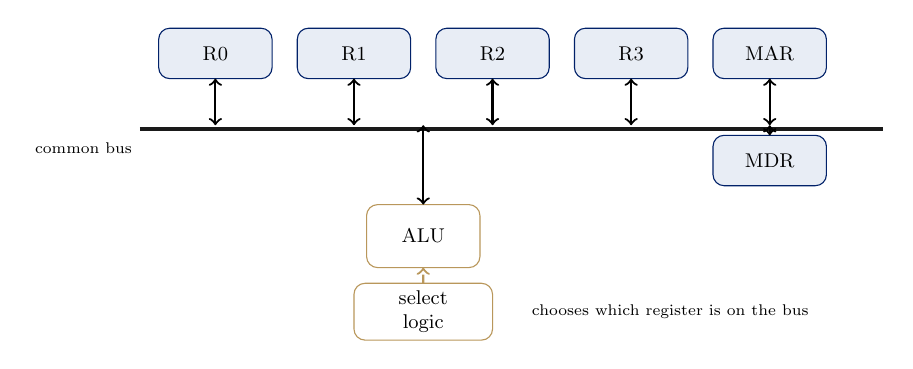
\begin{tikzpicture}[scale=0.80, transform shape,
      every node/.style={font=\small}]
    \draw[very thick, jet] (-1.2,0) -- (10.6,0);
    \node[font=\scriptsize, below left] at (-1.2,-0.1) {common bus};
    \node[draw=primary-blue, fill=light-bg, rounded corners,
          minimum width=1.8cm, minimum height=0.8cm, align=center] (R0) at (0,1.2) {R0};
    \node[draw=primary-blue, fill=light-bg, rounded corners,
          minimum width=1.8cm, minimum height=0.8cm, align=center] (R1) at (2.2,1.2) {R1};
    \node[draw=primary-blue, fill=light-bg, rounded corners,
          minimum width=1.8cm, minimum height=0.8cm, align=center] (R2) at (4.4,1.2) {R2};
    \node[draw=primary-blue, fill=light-bg, rounded corners,
          minimum width=1.8cm, minimum height=0.8cm, align=center] (R3) at (6.6,1.2) {R3};
    \foreach \x in {0, 2.2, 4.4, 6.6} { \draw[<->, thick] (\x,0.8) -- (\x,0.06); }
    \node[draw=primary-gold, fill=white, rounded corners,
          minimum width=1.8cm, minimum height=1.0cm, align=center] (ALU) at (3.3,-1.7) {ALU};
    \draw[<->, thick] (3.3,0.06) -- (3.3,-1.2);
    \node[draw=primary-blue, fill=light-bg, rounded corners,
          minimum width=1.8cm, minimum height=0.8cm, align=center] (MAR) at (8.8,1.2) {MAR};
    \node[draw=primary-blue, fill=light-bg, rounded corners,
          minimum width=1.8cm, minimum height=0.8cm, align=center] (MDR) at (8.8,-0.5) {MDR};
    \draw[<->, thick] (8.8,0.8) -- (8.8,0.06);
    \draw[<->, thick] (8.8,-0.1) -- (8.8,0.06);
    \node[draw=primary-gold, fill=white, rounded corners,
          minimum width=2.2cm, minimum height=0.8cm, align=center] (DEC) at (3.3,-2.9) {select\\logic};
    \draw[->, thick, primary-gold, dashed] (DEC.north) -- (3.3,-2.2);
    \node[font=\scriptsize, anchor=west] at (4.9,-2.9) {chooses which register is on the bus};
  \end{tikzpicture}
  \caption{The common bus system --- cf.\ Mano, \textit{Computer System Architecture}, 3rd ed., Fig.~5-4, p.129 (registers and memory on the common bus system). One shared path carries values among registers, ALU, and memory; a select unit (decoder) chooses which register drives the bus each cycle \cite{Mano1993_computer_system_architecture}.}
  \label{fig:common-bus}
\end{figure}

\subsection{Register-Selection Signals: SELA / SELB / SELD}

How does a transfer pick its source and destination? Mano's Table 8-1 (p.243) encodes the answer in three fields \cite{Mano1993_computer_system_architecture}. \texttt{SELA} names which register's contents go to the ALU's \emph{first} input; \texttt{SELB} names which register's contents go to the ALU's \emph{second} input; and \texttt{SELD} names \emph{which} register is loaded with the result.

The idea is that register selection is just \emph{encoded} in a few select bits and decoded into one-hot ``drive bus'' / ``load now'' signals. That is the whole trick behind moving values between registers without hard-wiring every pair.

\begin{example}[Copying \texttt{R1} $\gets$ \texttt{[R2]} over the common bus]
The transfer request is to copy the \emph{contents} of \texttt{R2} into \texttt{R1} (in the course's notation, the contents of a register X are written $[X]$). The bus-based mechanism is:
\begin{enumerate}
  \item \texttt{SELA} encodes ``\texttt{R2}'' --- R2's output enable goes high.
  \item \texttt{R2}'s contents are driven onto the common bus.
  \item \texttt{SELD} encodes ``\texttt{R1}'' --- R1's load-enable goes high.
  \item On the clock edge, \texttt{R1} captures whatever the bus holds: $R1 \gets [R2]$.
\end{enumerate}
No direct \texttt{R2}$\to$\texttt{R1} wire exists --- every transfer uses the bus plus two select signals. The same mechanism drives every register move and ALU operand.
\end{example}

\subsection{Socratic Check: Why Not Put \emph{Everything} in Registers?}

If registers are the fastest storage, why does a program put \texttt{X}, \texttt{A}, \texttt{B}, \texttt{C}, \texttt{D} in memory instead of keeping everything in \texttt{R0..Rn-1}? The answer has two parts. \bad{Registers are scarce}: a few dozen at most --- the program cannot keep megabytes of data there. And \bad{cost}: each register costs silicon area and consumes power; large register files are expensive. So registers are a \good{scratchpad for what is \emph{being} worked on}: values rest in memory (big, cheap, persistent) and are loaded into registers only while the ALU touches them.

\section{Stack Organization}
\label{sec:stack-organization}

\subsection{Motivation: How Do You Evaluate a Postfix Expression?}

Humans write \texttt{A + B}; machines with one ALU must feed it two operands. How would a calculator evaluate \texttt{A B +} if it could only look at the \emph{top} item of a scratch list --- no registers, no random access? The rule: read a value, \key{push} it; read an operator, \key{pop} the last two values, compute, \key{push} the result. The \emph{last} value pushed is the \emph{first} one taken back out --- \key{last-in, first-out} (LIFO). That is a \key{stack}. Many machines (HP calculators, the JVM) use exactly this model.

\begin{definitionbox}{Stack}
A stack is an ordered storage structure where all insertions and deletions happen at \emph{one end}, the \textbf{top}, addressed by a dedicated register \texttt{SP} (the \key{stack pointer}). Behavior is LIFO (Mano, Sec.~8-3, p.247) \cite{Mano1993_computer_system_architecture}.
\end{definitionbox}

Two operations manipulate the stack. \key{PUSH}: $SP \gets [SP] - 1$, then $M[SP] \gets$ operand --- store at the new top (the stack grows \emph{downward} toward lower addresses). \key{POP}: operand $\gets M[SP]$, then $SP \gets [SP] + 1$ --- remove the current top.

\begin{example}[PUSH and POP micro-transfers]
Suppose the stack contains \texttt{[? , 5 , 7]} with top at 7. \texttt{PUSH 9} $\Rightarrow$ stack \texttt{[? , 5 , 7 , 9]}; \texttt{POP} $\Rightarrow$ returns 9, and the stack is back to \texttt{[? , 5 , 7]}.
\end{example}

\begin{example}[\texttt{A + B} on a stack machine]
\begin{center}
\small
\begin{tabular}{@{}clp{4.2cm}p{4.2cm}@{}}
\toprule
\textbf{Step} & \textbf{Operation} & \textbf{Stack after (top right)} & \textbf{Effect} \\
\midrule
1 & \texttt{PUSH A} & \texttt{A} & value A stored at top \\
2 & \texttt{PUSH B} & \texttt{B A} & value B stored above A \\
3 & \texttt{ADD}    & \texttt{A+B} & pop B, pop A, push result \\
4 & \texttt{POP X}  & \emph{empty} & store top into \texttt{X} \\
\bottomrule
\end{tabular}
\end{center}
The \texttt{ADD} instruction names \emph{no operands at all} --- both come implicitly from the top of the stack. This is the \key{zero-address} instruction format we meet in Section~\ref{sec:instruction-formats}.
\end{example}

\subsection{Register Stack versus Memory Stack}

There are two hardware homes for a stack (Mano, Sec.~8-3, p.248) \cite{Mano1993_computer_system_architecture}. A \key{register stack} lives inside the CPU in a set of registers --- very fast, but only a handful of words (e.g.\ 64 words). A \key{memory stack} is a region of main memory, with \texttt{SP} holding the address of the current top --- as large as memory, but every PUSH/POP is a memory access.

Real machines choose memory stacks because function calls nest deeply (recursion); a few registers cannot hold the frames. Real ISAs keep \texttt{SP} in a register and store stack frames in memory --- registers are the pointer, memory is the stack. (P\&H's LEGv8 makes exactly this choice: \texttt{SP} is a dedicated register and the procedure-call convention pushes frames onto memory, Sec.~2.8, p.100) \cite{PattersonHennessy2017_computer_organization_design}.

\subsection{Socratic Check: Registers versus Stack as the Operand Home}

Both a register file and a stack can supply the ALU's operands. What does a stack force you to do that registers do not? \bad{Access is restricted}: you can only reach the \emph{top} --- no random access to \texttt{R0..Rn-1}-style slots mid-computation. \bad{Reordering costs}: to use a value that is buried, you must pop everything above it first (or shuffle). \good{But instructions shrink}: operands are implicit --- hence the compact \key{zero-address} format. Compilers love the compactness; hardware pays with restricted access.

\section{Instruction Formats}
\label{sec:instruction-formats}

\subsection{Motivation: What Must an Instruction Say?}

The CPU must be told \emph{what} to do and \emph{where} the operands are. How much ``where'' information must a machine instruction physically carry? At minimum, an \key{opcode} --- which operation (\texttt{ADD}, \texttt{LOAD}, \dots). Beyond that, \emph{addresses} of operands and results --- and each address costs bits in the instruction word. The trade-off is fundamental: \key{more addresses per instruction} $\Rightarrow$ more work done per instruction but \key{longer instructions}; fewer addresses $\Rightarrow$ compact but \key{more instructions} (and the hardware must know where the operands are implicitly).

\begin{definitionbox}{Instruction Format}
An instruction format is the layout of an instruction word: an \textbf{opcode} field naming the operation, followed by zero or more \textbf{address/operand} fields naming where operands and results live (Mano, Sec.~8-4, p.255) \cite{Mano1993_computer_system_architecture}.
\end{definitionbox}

Fields are fixed-width bits; the opcode width sets an upper bound on how many distinct instructions the ISA can name. Address fields can name registers (short, cheap) or memory locations (long, flexible) --- Week 5 turns those fields into real addresses via \key{addressing modes}. Patterson \& Hennessy's LEGv8 shows the fixed-width field idea concretely: instructions are laid out in a handful of formats (R/I/IS/B/CB/IM), each with fixed fields, and the opcode width bounds the instruction count (P\&H, Sec.~2.5, p.82) \cite{PattersonHennessy2017_computer_organization_design}.

\subsection{The Four Format Families}

As the operand count falls, instructions get shorter but the machine must find operands \emph{implicitly} (accumulator or stack top). Figure~\ref{fig:format-families} shows the four families as horizontal word layouts.

\begin{figure}[h]
  \centering
  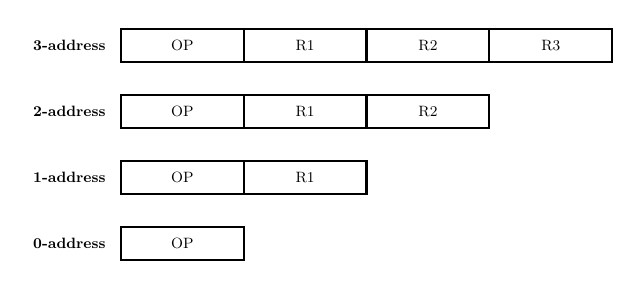
\begin{tikzpicture}[scale=0.6, transform shape,
      every node/.style={font=\small}]
    \draw[thick] (0,0) rectangle (10.4,-0.7);
    \draw[thick] (2.6,0) -- (2.6,-0.7);  \draw[thick] (5.2,0) -- (5.2,-0.7);
    \draw[thick] (7.8,0) -- (7.8,-0.7);
    \node at (1.3,-0.35) {OP}; \node at (3.9,-0.35) {R1};
    \node at (6.5,-0.35) {R2}; \node at (9.1,-0.35) {R3};
    \node[left] at (-0.2,-0.35) {\textbf{3-address}};
    \draw[thick] (0,-1.4) rectangle (7.8,-2.1);
    \draw[thick] (2.6,-1.4) -- (2.6,-2.1);  \draw[thick] (5.2,-1.4) -- (5.2,-2.1);
    \node at (1.3,-1.75) {OP}; \node at (3.9,-1.75) {R1}; \node at (6.5,-1.75) {R2};
    \node[left] at (-0.2,-1.75) {\textbf{2-address}};
    \draw[thick] (0,-2.8) rectangle (5.2,-3.5);
    \draw[thick] (2.6,-2.8) -- (2.6,-3.5);
    \node at (1.3,-3.15) {OP}; \node at (3.9,-3.15) {R1};
    \node[left] at (-0.2,-3.15) {\textbf{1-address}};
    \draw[thick] (0,-4.2) rectangle (2.6,-4.9);
    \node at (1.3,-4.55) {OP};
    \node[left] at (-0.2,-4.55) {\textbf{0-address}};
  \end{tikzpicture}
  \caption{The four instruction-format families --- cf.\ Mano, \textit{Computer System Architecture}, 3rd ed., Sec.~8-4, p.255: as the operand count falls, instructions get shorter but the machine must find operands implicitly \cite{Mano1993_computer_system_architecture}.}
  \label{fig:format-families}
\end{figure}

\textbf{Three- and two-address forms.} The 3-address form, \texttt{ADD R1, R2, R3} $\Rightarrow$ $R1 \gets [R2]+[R3]$, makes operands and destination all explicit --- the most flexible, longest form. The 2-address form, \texttt{ADD R1, R2} $\Rightarrow$ $R1 \gets [R1]+[R2]$, lets the first field double as one operand \emph{and} the result destination --- this is \key{destructive}: the old value of \texttt{R1} is lost. Fewer fields $\Rightarrow$ shorter instructions and smaller programs, at the cost of destroying one operand and needing explicit copy instructions.

\textbf{One- and zero-address forms.} The 1-address (accumulator) form, \texttt{ADD A} $\Rightarrow$ $AC \gets [AC]+[A]$, always uses the accumulator \texttt{AC} as one operand (named by no field); the single field names the other operand (usually memory). The 0-address (stack) form, \texttt{ADD} $\Rightarrow$ pop two, push sum, carries \emph{only} the opcode; every operand is implicit from the stack top. This is extreme compactness, but every non-stack access needs explicit \texttt{PUSH}/\texttt{POP} instructions.

\subsection{Worked Examples: $X = (A+B)\times(C+D)$ in Every Format}

The running thread makes the trade-off countable. In the \textbf{three-address} format the expression compiles to 3 instructions, operands all named:
\begin{example}[3-address: \texttt{X = (A+B)$\times$(C+D)}]
\begin{center}
\small
\begin{tabular}{@{}lcp{7cm}@{}}
\toprule
\textbf{Instruction} & \textbf{Effect} & \textbf{Notes} \\
\midrule
\texttt{ADD R1, A, B} & $R1 \gets A + B$ & operands and result all named \\
\texttt{ADD R2, C, D} & $R2 \gets C + D$ & \\
\texttt{MUL X, R1, R2} & $X \gets R1 \times R2$ & \\
\bottomrule
\end{tabular}
\end{center}
3 instructions; each carries three addresses --- wide words, but the program is short and needs no extra data movement.
\end{example}

The \textbf{two-address} format needs 5 instructions because the destructive form requires copies:
\begin{example}[2-address: the same expression]
\begin{center}
\small
\begin{tabular}{@{}llcp{7cm}@{}}
\toprule
\textbf{Instruction} & \textbf{Effect} & \textbf{Why} \\
\midrule
\texttt{MOV R1, A} & $R1 \gets A$ & explicit copy, since \texttt{ADD} overwrites \\
\texttt{ADD R1, B} & $R1 \gets R1 + B$ & \\
\texttt{MOV R2, C} & $R2 \gets C$ & \\
\texttt{ADD R2, D} & $R2 \gets R2 + D$ & \\
\texttt{MUL X, R1} & $X \gets R1 \times R2$ & R2 is the implicit second operand \\
\bottomrule
\end{tabular}
\end{center}
5 instructions vs.\ 3 --- the 2-address format is cheaper per instruction but needs \key{extra copy instructions} because \texttt{ADD} is destructive.
\end{example}

The \textbf{one-address} (accumulator) format needs 7 instructions; a temporary \texttt{T} in memory is required because the accumulator cannot hold two partial results at once:
\begin{example}[1-address: the same expression]
\texttt{LOAD A; ADD B; STORE T; LOAD C; ADD D; MUL T; STORE X} --- with a temporary \texttt{T} in memory because the accumulator cannot hold two partial results at once.
\end{example}

The \textbf{zero-address} (stack) format needs 8 instructions, the most of any format, but each is the shortest possible:
\begin{example}[0-address: the same expression]
\texttt{PUSH A; PUSH B; ADD; PUSH C; PUSH D; ADD; MUL; POP X} --- shortest instructions, but the most of them.
\end{example}

\subsection{The Four Formats Side by Side}

Table~\ref{tab:format-comparison} summarizes the four families. Same expression, four formats: 3, 5, 7, and 8 instructions. More addresses per instruction $\Rightarrow$ fewer instructions but wider words; fewer addresses $\Rightarrow$ more instructions but compact.

\begin{table}[h]
\centering
\small
\renewcommand{\arraystretch}{1.15}
\begin{tabular}{@{}p{1.8cm}p{2.4cm}p{4.0cm}p{2.2cm}p{2.6cm}@{}}
\toprule
\textbf{Format} & \textbf{Example} & \textbf{Program size for }$X=(A{+}B)\times(C{+}D)$ & \textbf{Operand access} & \textbf{Typical use} \\
\midrule
3-address & \texttt{ADD R1,R2,R3} & 3 instr., wide words & all explicit & register ISAs (RISC) \\
2-address & \texttt{ADD R1,R2}    & 5 instr. + copies     & one destroyed      & older CISC \\
1-address & \texttt{ADD A}        & 7 instr., needs temps & accumulator        & simple CPUs \\
0-address & \texttt{ADD}          & 8 instr., compact    & stack top          & stack machines, JVM \\
\bottomrule
\end{tabular}
\caption{Instruction formats side by side --- cf.\ Mano, \textit{Computer System Architecture}, 3rd ed., Sec.~8-4, p.255 \cite{Mano1993_computer_system_architecture}.}
\label{tab:format-comparison}
\end{table}

\section{Instruction Cycle}
\label{sec:instruction-cycle}

\subsection{Motivation: Who Runs the Show, Step by Step?}

\texttt{ADD R1, A} sits in memory. For it to take effect, the CPU must bring the instruction in, understand it, collect \texttt{[R1]} and \texttt{[A]}, add, and store back. The answer is a fixed skeleton --- the \key{instruction cycle} --- that the control unit runs over and over, once per instruction. The skeleton is the \emph{same} for every instruction; only the \key{execute} phase differs by opcode.

\begin{definitionbox}{Instruction Cycle}
The fixed sequence of phases --- fetch, decode, execute --- the control unit repeats once per instruction; only the execute phase varies with the opcode.
\end{definitionbox}

\subsection{The Cycle: Fetch, Decode, Execute}

Fetch $\to$ decode $\to$ execute is the standard instruction-cycle skeleton (Hamacher, \textit{Computer Organization}, Ch.~7; standard treatment) \cite{Hamacher2002_computer_organization}. Figure~\ref{fig:instruction-cycle} shows it as a loop.

\begin{figure}[h]
  \centering
  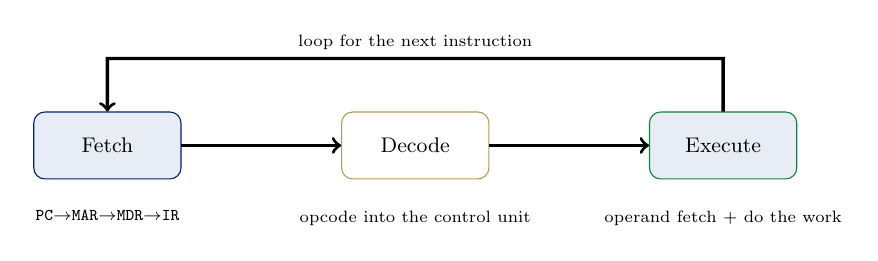
\begin{tikzpicture}[scale=0.85, transform shape,
      every node/.style={font=\small}]
    \node[draw=primary-blue, fill=light-bg, rounded corners,
          minimum width=2.2cm, minimum height=1.0cm, align=center] (F) at (0,0) {Fetch};
    \node[draw=primary-gold, fill=white, rounded corners,
          minimum width=2.2cm, minimum height=1.0cm, align=center] (D) at (4.6,0) {Decode};
    \node[draw=positive, fill=light-bg, rounded corners,
          minimum width=2.2cm, minimum height=1.0cm, align=center] (E) at (9.2,0) {Execute};
    \draw[->, very thick] (F.east) -- (D.west);
    \draw[->, very thick] (D.east) -- (E.west);
    \draw[->, very thick] (E.north) -- (9.2,1.3) -- (0,1.3) -- (F.north);
    \node[font=\scriptsize, above] at (4.6,1.3) {loop for the next instruction};
    \node[font=\scriptsize, below] at (0,-0.85) {\texttt{PC}$\to$\texttt{MAR}$\to$\texttt{MDR}$\to$\texttt{IR}};
    \node[font=\scriptsize, below] at (4.6,-0.85) {opcode into the control unit};
    \node[font=\scriptsize, below] at (9.2,-0.85) {operand fetch + do the work};
  \end{tikzpicture}
  \caption{The instruction cycle --- fetch, decode, execute --- as a loop (Hamacher, \textit{Computer Organization}, Ch.~7; standard treatment) \cite{Hamacher2002_computer_organization}.}
  \label{fig:instruction-cycle}
\end{figure}

\subsection{The Fetch Phase, Step by Step}

The fetch phase moves the next instruction from memory into the CPU (\texttt{PC} knows where the next instruction lives):
\begin{itemize}
  \item \texttt{MAR} $\gets$ \texttt{[PC]} --- remember the address.
  \item Initiate a memory \emph{read} at \texttt{MAR}.
  \item \texttt{MDR} $\gets$ \emph{memory data} --- the instruction word comes back into the CPU.
  \item \texttt{IR} $\gets$ \texttt{[MDR]} --- the instruction now sits in the instruction register.
  \item \texttt{PC} $\gets$ \texttt{[PC]} $+ 1$ --- prepare the \emph{next} fetch.
\end{itemize}

Why these registers? \texttt{PC} holds the next address, \texttt{MAR} pins it during the access, \texttt{MDR} buffers the incoming word, \texttt{IR} holds the current instruction while it is decoded. Each register exists for \emph{one} reason in the cycle.

\subsection{The Decode and Execute Phases}

\textbf{Decode.} The opcode bits of \texttt{IR} tell the control unit \emph{which} operation this is --- the unit then selects the right sequence of control signals (exactly what we build in Weeks~6--7).

\textbf{Execute} is the operand-dependent part. If a memory operand is needed, its address is resolved (addressing modes, Week 5) and the operand fetched into a register. The ALU performs the operation; the result is written to the destination named in the instruction. The \emph{number} of execute steps varies by instruction --- fetch is fixed, execute is not.

\begin{example}[One full cycle for \texttt{ADD R1, A}]
\begin{center}
\small
\begin{tabular}{@{}cp{3.4cm}p{3.6cm}p{3.4cm}@{}}
\toprule
\textbf{Phase} & \textbf{Register activity} & \textbf{Memory / ALU} & \textbf{State} \\
\midrule
Fetch &
  \texttt{MAR}$\gets$\texttt{[PC]}; \texttt{MDR}$\gets$instr.; \texttt{IR}$\gets$\texttt{[MDR]}; \texttt{PC}$\gets$\texttt{[PC]}$+1$ &
  read instruction word &
  instruction in \texttt{IR} \\
Decode &
  \texttt{IR} opcode $\to$ control unit &
  --- &
  operation identified \\
Execute &
  operand \texttt{[A]} fetched; \texttt{AC}$\gets$\texttt{[AC]}+\texttt{[A]} &
  read operand; ALU adds &
  result in \texttt{AC} \\
\bottomrule
\end{tabular}
\end{center}
The same three phases run for every instruction --- only the execute row changes. This is the loop the CPU is always inside.
\end{example}

\subsection{Types of Operands}

What the fields of an instruction can name (Hamacher, Ch.~7; standard treatment) \cite{Hamacher2002_computer_organization}:
\begin{itemize}
  \item \key{Addresses}: a location in memory (used by \texttt{LOAD}, \texttt{STORE}, \texttt{BRANCH}).
  \item \key{Numbers}: integer or floating-point values the ALU computes on.
  \item \key{Characters}: text --- usually ASCII/Unicode codes stored in a byte or halfword.
  \item \key{Logical data}: bit patterns --- each bit is its own value; operations like \texttt{AND}, \texttt{OR}, \texttt{XOR}, \texttt{shift} work bitwise.
\end{itemize}

Why this matters: the \emph{type} determines how the ALU wires the bits. A branch needs the address, an integer add needs the value, a shift needs the bit mask. The opcode says which interpretation applies. (P\&H's LEGv8 makes the same point in its operand taxonomy --- registers, memory, constants --- Sec.~2.3, p.67, and the branch/decision instructions of Sec.~2.7, p.93) \cite{PattersonHennessy2017_computer_organization_design}.

\subsection{Socratic Check: Tying the Week Together}

For \texttt{ADD R1, A} on an accumulator machine: which register holds the next instruction's address, which holds the current instruction, and where do the two operands of the ADD come from? \texttt{PC} points at the next instruction; \texttt{IR} holds the current one after fetch. The first operand is \texttt{AC} (the accumulator --- the implicit operand of the 1-address format). The second operand is memory location \texttt{A}, fetched during execute. Every piece of this answer came from the preceding sections --- the registers, the formats, and the cycle are one connected machine.

\section{Synthesis and Summary}
\label{sec:synthesis}

\subsection{The Three Threads Meet}

Storage spaces and formats are two sides of one choice. \key{Registers}: fast, explicit, random access --- buys the wide 3-address format. \key{Stack}: compact, restricted, implicit --- buys the 0-address format. The instruction cycle is the \emph{glue}: it steps whichever format the ISA chose, through the same fetch/decode/execute skeleton.

The running thread closes: $X = (A+B)\times(C+D)$ ran in 3, 5, 7, or 8 instructions depending on the format --- and each of those instructions then lives through one full fetch--decode--execute cycle.

\subsection{Bridge to Week 5}

What we built this week: the CPU's storage (registers --- fast scratchpad; stack --- LIFO operand home; memory --- big and slow); four instruction formats with a counted cost per format; and the fetch--decode--execute cycle with the four types of operands. What is still missing: we wrote ``\texttt{ADD R1, A}'' and said ``operand \texttt{[A]} is fetched'' --- but we never said \key{how} the field \texttt{A} turns into the actual location of the operand. That is \key{addressing modes}, next week --- together with the datapath (buses) that actually moves the values.

\subsection{Summary}

\textbf{Register organization:} registers are the one-cycle scratchpad; transfers happen over a common bus selected by \texttt{SELA}/\texttt{SELB}/\texttt{SELD}. \textbf{Stack organization:} \texttt{SP} addresses a LIFO top; PUSH/POP with $\pm 1$ on \texttt{SP}; register stacks are fast, memory stacks are large. \textbf{Instruction formats:} 3-, 2-, 1-, 0-address --- the address count trades instruction width against program size (3 vs.\ 5 vs.\ 7 vs.\ 8 instructions for one expression). \textbf{Instruction cycle:} fetch (\texttt{PC}$\to$\texttt{MAR}$\to$\texttt{MDR}$\to$\texttt{IR}, \texttt{PC}${+}1$), decode, execute. \textbf{Operand types:} addresses, numbers, characters, logical data --- the opcode picks the interpretation.

\bibliographystyle{plain}
\bibliography{../../Bibliography_base}

\end{document}
